\documentclass{report}
%\usepackage[utf8]{inputenc}
\usepackage{outlines}
\usepackage{fancyvrb}
\usepackage[round, authoryear]{natbib}
%\bibliographystyle{plainnat}
\usepackage[breaklinks,colorlinks,linkcolor=black,citecolor=blue,urlcolor=blue, anchorcolor=blue,bookmarks=true]{hyperref}
\usepackage[a4paper, total={6in, 10in},top=1.2in, bottom=0.7in, includefoot]{geometry}
\usepackage{adjustbox}
%$\usepackage[export]{adjustbox}
\usepackage{graphicx}
\graphicspath{{./images/}}
\usepackage{booktabs}
\usepackage{multirow}
\usepackage{hyperref}
\usepackage{comment}
\usepackage{listings}
\usepackage{xcolor}

\usepackage{pdfpages}

%New colors defined below
\definecolor{codegreen}{rgb}{0,0.6,0}
\definecolor{codegray}{rgb}{0.5,0.5,0.5}
\definecolor{codepurple}{rgb}{0.58,0,0.82}
\definecolor{backcolour}{rgb}{0.95,0.95,0.92}

%Code listing style named "mystyle"
\lstdefinestyle{mystyle}{
  backgroundcolor=\color{backcolour},   commentstyle=\color{codegreen},
  keywordstyle=\color{magenta},
  numberstyle=\tiny\color{codegray},
  stringstyle=\color{codepurple},
  basicstyle=\ttfamily\footnotesize,
  breakatwhitespace=false,         
  breaklines=true,                 
  captionpos=b,                    
  keepspaces=true,                 
  numbers=left,                    
  numbersep=5pt,                  
  showspaces=false,                
  showstringspaces=false,
  showtabs=false,                  
  tabsize=2
}

%"mystyle" code listing set
\lstset{style=mystyle}

%to do list with progress

\usepackage{enumitem,amssymb,amsmath}
\newlist{todolist}{enumerate}{2}
\setlist[todolist]{label=$\square$}
\usepackage{pifont}
\newcommand{\cmark}{\ding{51}}%
\newcommand{\xmark}{\ding{55}}%
\newcommand{\done}{\rlap{$\square$}{\raisebox{2pt}{\large\hspace{1pt}\cmark}}%
\hspace{-2.5pt}}
\newcommand{\wontfix}{\rlap{$\square$}{\large\hspace{1pt}\xmark}}
\usepackage{fontawesome}
 %\usepackage{algorithm}
\usepackage[ruled,vlined]{algorithm2e}
%\usepackage{algorithmic}
\usepackage{float}
\usepackage{arevmath}     % For math symbols
\usepackage[noend]{algpseudocode}

\usepackage{cancel} %strike through
\usepackage[normalem]{ulem}
%\newcommand{\done}{\rlap{$\square$}{\raisebox{2pt}{\large\hspace{1pt}\cmark}}%
\usepackage{csvsimple}
\title{Commonsense Knowledge Graph Completion }
\author{Chunhua Liu}
%\date{Version 0.3,  21 April, 2020}


\begin{document}

    \maketitle
    
%    \begin{abstract}
        
%    \end{abstract}
    
    \thispagestyle{empty}
    \tableofcontents
    \thispagestyle{empty}
    \newpage
    \setcounter{page}{1}
    
%\tableofcontents
%% 符号对照表
%\input{data/denotation}

%%% 正文部分
\chapter{2020-07-07}

\textbf{Check list for data creation}
\begin{enumerate}
    \item Sampling order 
    \item Ensure the nodes and triples num to be close 
    \item Output degree of the test and valid graph 
    \item Output the entity frequency on sampled graph, SWOW and ConceptNet
    \item If h and t hold n relations, add all the relations to SWOW
    \item Ensure the content of the final written triples is consistent with the orginal one
\end{enumerate}

\section{Dataset Creation}
\subsection{Statistics of Dataset}
\begin{table}
\centering
    \begin{tabular}{l|llllll}
	\toprule
	 Category & File name & Triples & Entities & Relations & avg.Degree & Density \\
	\midrule
	 CN-100K & cn\_100k\_train\_valid\_test & 102,400 & 78,334 & 34 & 1.275  &1.7e-5 \\
     SWOW & swow\_freq2.filter & 413,481 & 34,829 & 1 &  11.871 & 3.4e-4 \\
    \hline
	 Overlap & overlap\_triples & 8,122 & 4,006 & 33 &  \\
	 Overlap & overlap\_entities &  & 8,382 &  &  \\
    \hline
    Train & rel\_triples1 & 100,162 & 78,173 & 34 & 1.251 & 1.6e-5\\
	Train & rel\_triples2 & 413,504 & 34,813 & 34 & 11.864 & 3.41e-4\\
	Train & ent\_links\_train &  & 6,600 &  \\
	Train & rel\_links &  &  & 33 & \\
    \hline
	Test & rel\_triples\_test & 1,125 & 889 & 27 & 1.165 & 1.42e-3 \\
	Test & ent\_links\_test &  & 889 &  \\
    \hline
	Valid & rel\_triples\_valid & 1,110 & 893 & 29 & 1.159 & 1.39e-3\\
	Valid & ent\_links\_valid &  & 893 &  \\
	\bottomrule
\end{tabular}
\caption{\label{tab:dataset_statistics} Data Statistics for newly created dataset.}
\end{table}


node degree distribution of valid and test 
learning curves on current model (current versionm, still need to debug)


\subsection{Procedures of creating dataset}
\clearpage
\begin{algorithm}[H]
    \SetAlgoLined
    \LinesNumbered
    \KwData{Triples from ConceptNet and SWOW}
    \KwResult{Triples for train $\mathcal{T}_{tr}$, valid $\mathcal{T}_v$, test $\mathcal{T}_{te}$}
    \KwResult{Overlap entities for train, valid, test alignment task}
    \KwResult{Overlap relations for train, valid, test} 
    Initilize overlap triples $\mathcal{T}_o= set()$  \\
    Initilize overlap nodes $\mathcal{N}_{o} = set()$  \\
    Build a directional CN-Graph $\mathcal{G}_c$ \\
    Build a directional SW-Graph $\mathcal{G}_s$ \\
    \For{$(h,t) \gets \mathcal{G}_s$} {
        \If{$(h,t) \in \mathcal{G}_c $} {
            \For{$r \gets \mathcal{G}_{c}(h,t)$}{ %\Comment*{Multiple relations may hold}
                 $\mathcal{T}_o \gets (r, h, t)$ \\ 
                 $\mathcal{N}_o \gets (h, t)$ \\
                 $\mathcal{G}_s \gets (r, h, t) $
            }
        } 
    }
    Sample 3000 nodes from $\mathcal{N}_o$ and shuffle them \\
    Split 3000 nodes into 2 sets, $\mathcal{N}_t, \mathcal{N}_v$ for sampling valid and test respectively \\
    \For {$ (r, h, t) \in \mathcal{E}_o$}{
        \If{$ (h,t) \in \mathcal{N}_t $}{
            $\mathcal{N}_t \gets (r, h, t)$
        }
        \If{$ (h,t) \in \mathcal{N}_v $}{
            $\mathcal{N}_v \gets (r, h, t)$
        }
    }

    \caption{\label{algo:create_alignment_dataset} Procedures of creating aligned dataset}
\end{algorithm}

\textbf{Code Checklist}
\begin{enumerate}
    \item Data
        \begin{enumerate}
            \item \sout{Generate negative samples for test and valid triples}
        \end{enumerate}
    \item  Evaluation 
        \begin{enumerate}
            \item  Compare my code with the others's to see whether there is any different
             \item  \faCheckSquareO Add filter rank code. \\ Purpose of filtered rank: For a given $(h,r)$ in the test set, we will compute the score with all the other entitities in the cadidate pool, e.g., $(h,r,t^{\prime})$, which could possibly be a true triple in the train, valid, test sets, and gets a higher score than the golden $t$, and lower the rank of $t$, which is unfair. So the way of removing  all the possible true triples from the corrupted triple list is called \textit{filtered rank}, and the other one is called \textit{raw rank}.  (see explinations from \cite{Bordes2013TransENIPS,Dettmers2018conve})
            \item \faCheckSquareO Debug the code of restoring a trained model for re-testing relation classifier
            \item  \faCheckSquareO Measure alignment in both directions 
            \item Evaluate the dev and test with mini-batch
        \end{enumerate}
    \item  Training
        \begin{enumerate}
            \item \faCheckSquareO Set FLAG for training with maxinum epoch or early stoping 
            \item \faCheckSquareO Use $0.5*(align\_hits1 + completion\_hits1)$ or $0.5*(align\_mrr + completion\_mrr)$ as the early stopping criteria 
            \item \faCheckSquareO If early stopping, save the model with the best performance
            \item If early stopping, restore and test the saved model with the best performance
            \item If early stopping, visualize the curves of stopping criteria
            \item Sort out code, make sure the alignment and completion code to be consistent
            \item Add regularizatons for weight parameters in relation classifier
        \end{enumerate}
    \item  Model
        \begin{enumerate}
            \item Make use of both embeddings learnt from CN and SW when doing evaluation. 
        \end{enumerate}
\end{enumerate}


%relation_classes can be removed and replace it with id_relations_dict




\include{data/2020-06-30}
\chapter{2020-06-23}

\textbf{Check List}
\begin{enumerate}
    \item \faCheckSquareO Figure out why `NAN' appears during training. \\
        A: the scores for some relation types are too small and caused the underflow when apply log function to them. A small number $\epsilon =1e-9$ is added to the scores for numerical stable.
    \item Debug the relation classifier \\
    For now, when $\beta_1$ is increased, the relation prediction accuracy become higher, but the alignment and completion performances dropped.  Try to figure out why, the code problem or the idea problem?
    Try to make the model and task to be simple to debug the relation classifier. 
    \begin{enumerate}
        \item \faCheckSquareO Try simpler version of dataset, e.g., two relaiton types.
        \item Observe some prediction outputs for alignment rank, completion rank, and relation prediction (both training and valid). 
    \end{enumerate}
    
    \item Relation classification overfitting: try different training strategy to alleviate the problem. 
    \begin{enumerate}
        \item \faCheckSquareO Play with hyperparameters: lr, batch\_size, and training\_epoch. 
        \item \faCheckSquareO Pretrain the relation classifier.
        \item \faCheckSquareO Train the relation classifier every K ($K$ \textgreater $1$) epoch instead of every epoch. 
    \end{enumerate}
\end{enumerate}

\section{Train 2 relation types}
When I was doing the experiments of learning only two relation types and visualizing the correlations between rel-acc and other metrics (hits@N, mr, mrr), I noticed that the prvious conclusion: ``\textbf{when rel-acc goes up, the other metrics go down}" is not completely correct (see Figure~\ref{fig:iptranse_C_S_V7_lineplot_metrics}). The  vibration at high rel-acc is because of more datapoints. From these curves, we can see when rel-acc is high, the other metrics could either high or low. It seems that there is no positive relationships between rel-acc and other metrics. 
Although I haven't figure out why, it gives me a hint that I can train them separately. %That is, we can first train the relaiton classifier to reach a decent rel-acc, and then reduce the frequency of updating parameteres in relation classifier. 
So, I made the following modifications for training the relation classifier:
\begin{enumerate}
    \item Separate the training process of 1) learning entity and relation embedding matrices, and 2) learning relation types. Then two optimizers are used to train two parts separately (previous: losses are added into one total loss and train it with one optimizer.)  
    \item The relation classifier is trained along with the embedding matrices at first N epoches. After that, it's updated every K epoches to avoid overfitting. This can ensure the relation classifier is well trained and also reduce the overfitting problem (see Algorithm~\ref{algo:asynchronously_training}).
\end{enumerate}

    The key difference is the gradients from the margin loss $L_e$ for triples  (see Figure~\ref{fig:model_architecture}) to the parameter $\theta$ in the relation classifier are cut down. So $\theta$ is only updated by $L_r and L_p$. 

\begin{algorithm}[H]
    \SetAlgoLined
    \KwIn{Triples from ConceptNet and SWOW}
    \KwIn{Aligned entity seeds}
    \KwIn{$N, M$ signify the max trining epoch for $L_e$ and $L_{rp}$, $N \geq M $. $K$ denotes an int number.}
    \KwResult{Entity embedding matrix $\mathbf{E}$, relation embedding matrix $\mathbf{R}$}
    \KwResult{Relation type classifier with parameter $\theta$}
    %$L_{rp} \gets \beta_1*L_r + \beta_2*L_p$\;
     initialization\;
     \For{$i \gets 0$ \textbf{to} $N$} {
            \eIf{$i < M$} {
                Update $\theta$
            } {
             \If{$ i \geq  M \vee i \% K =0$} {
                Update $\theta$ } 
            }
                Update $\mathbf{E}, \mathbf{R}$
      }
    \caption{\label{algo:asynchronously_training} Asynchronously trainining embedding matrices and relation types}
    \end{algorithm}

    \begin{figure}[!ht]
        \centering
        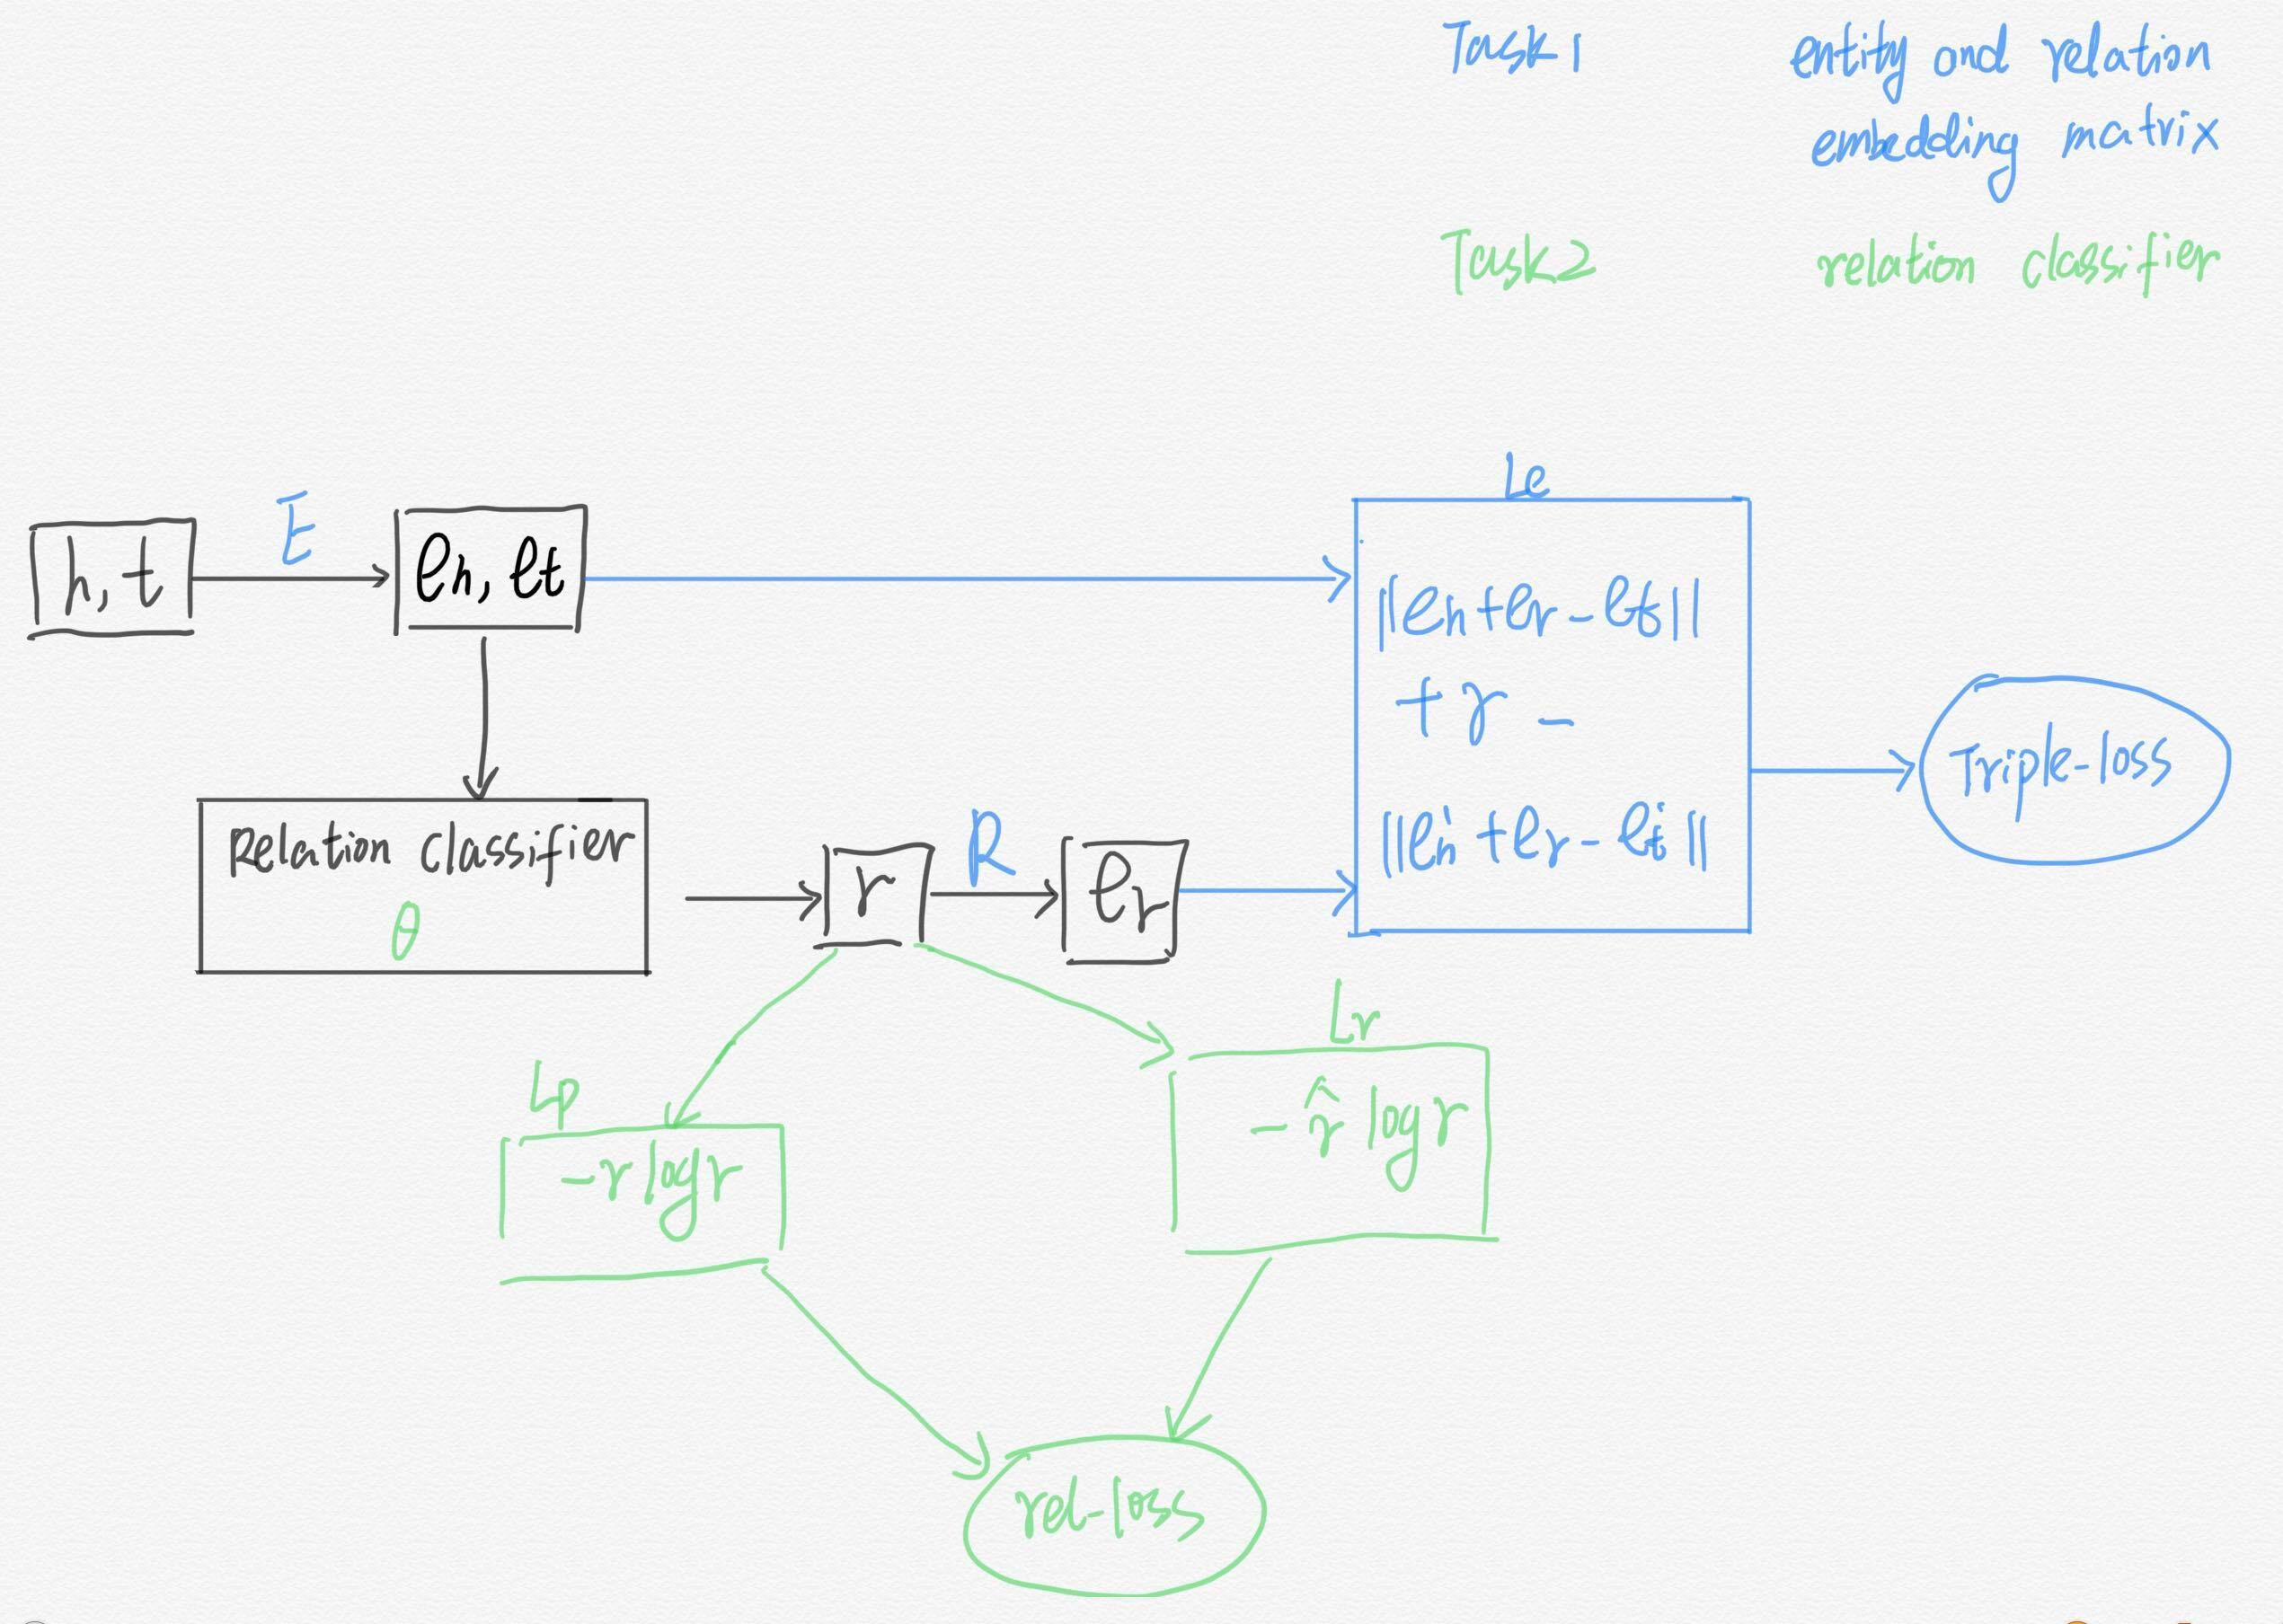
\includegraphics[width=\linewidth]{0623/model_architecture.jpg}
        \caption{\label{fig:model_architecture} The data flow in the model.}
    \end{figure}
\begin{figure}[H]
    \centering
    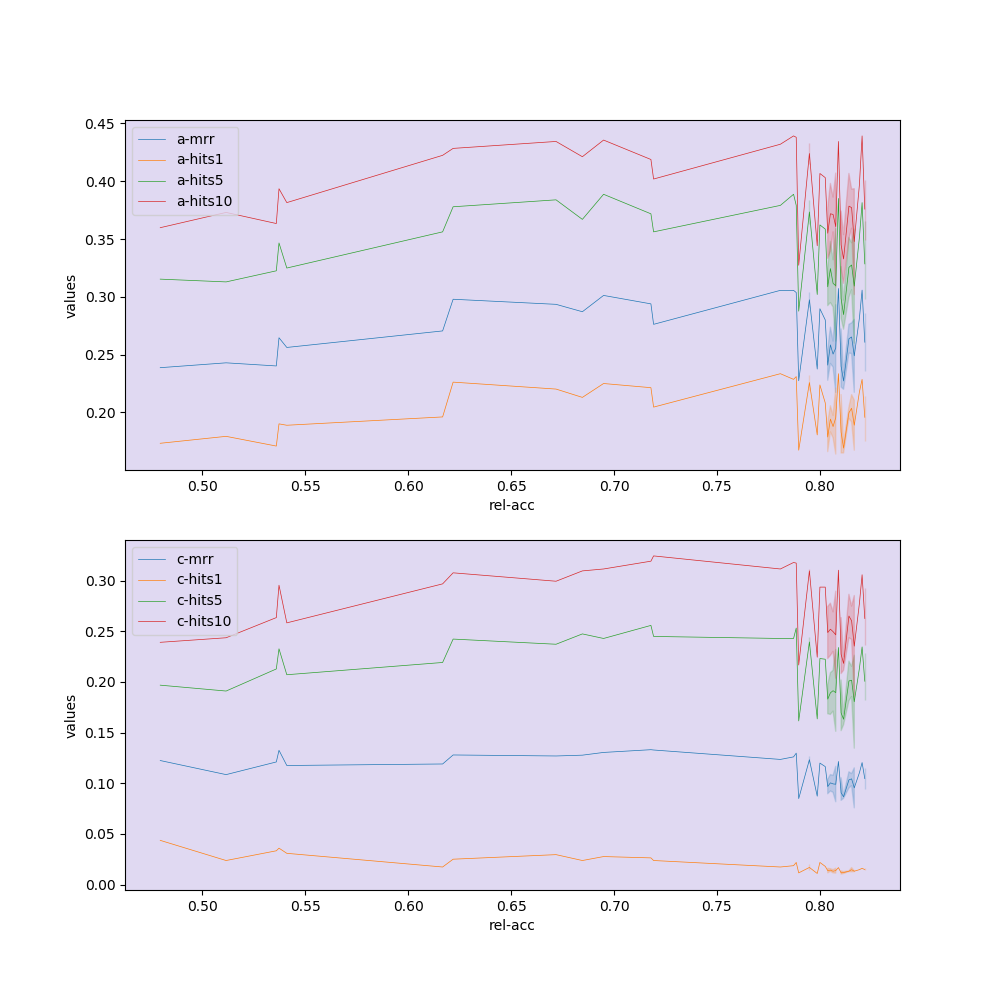
\includegraphics[width=\linewidth]{0623/iptranse_C_S_V7_lineplot_metrics.png}
    %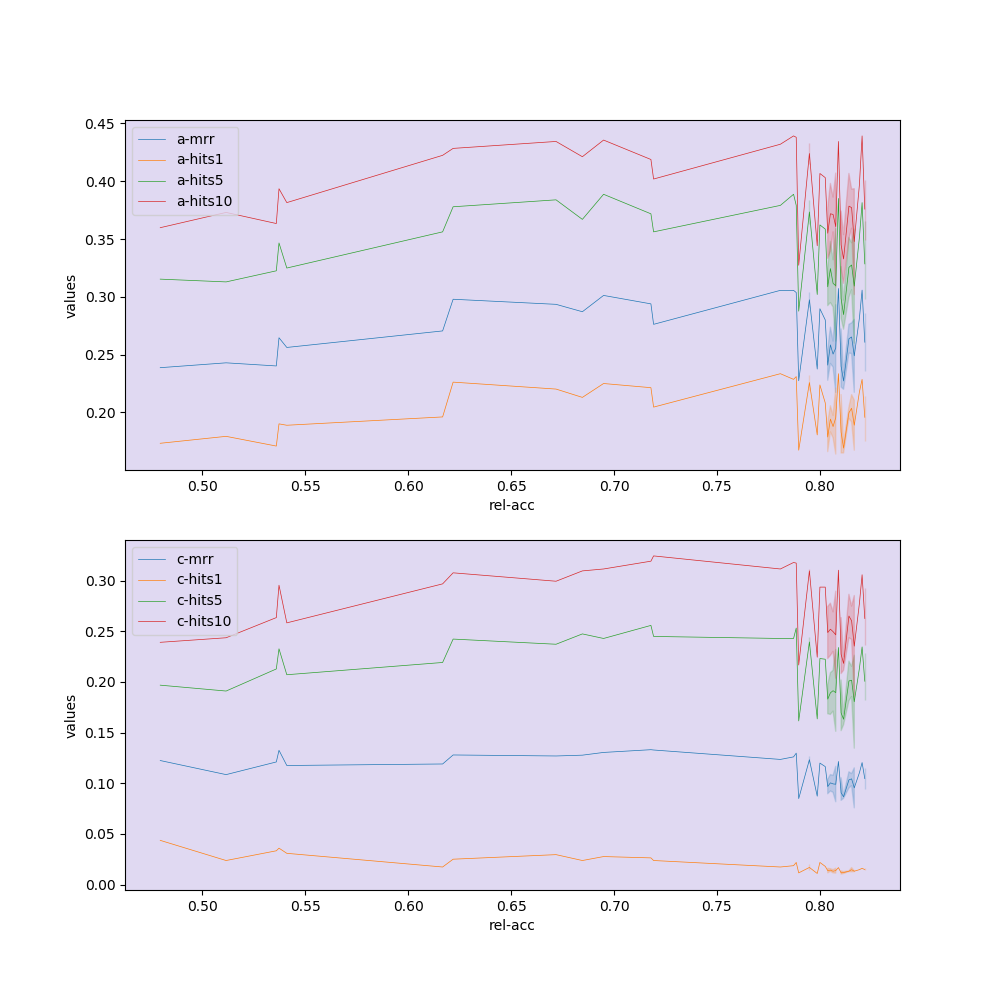
\includegraphics[scale=0.5]{0623/iptranse_C_S_V7_lineplot_metrics.png}
    \caption{\label{fig:iptranse_C_S_V7_lineplot_metrics} Correlations between rel-acc and other metrics. Embedding matrices and relations types are optimized with one optimizer. Parameters in relation classifier are updated with embedding matrices at every epoch.}
\end{figure}

\begin{figure}[H]
    \centering
    %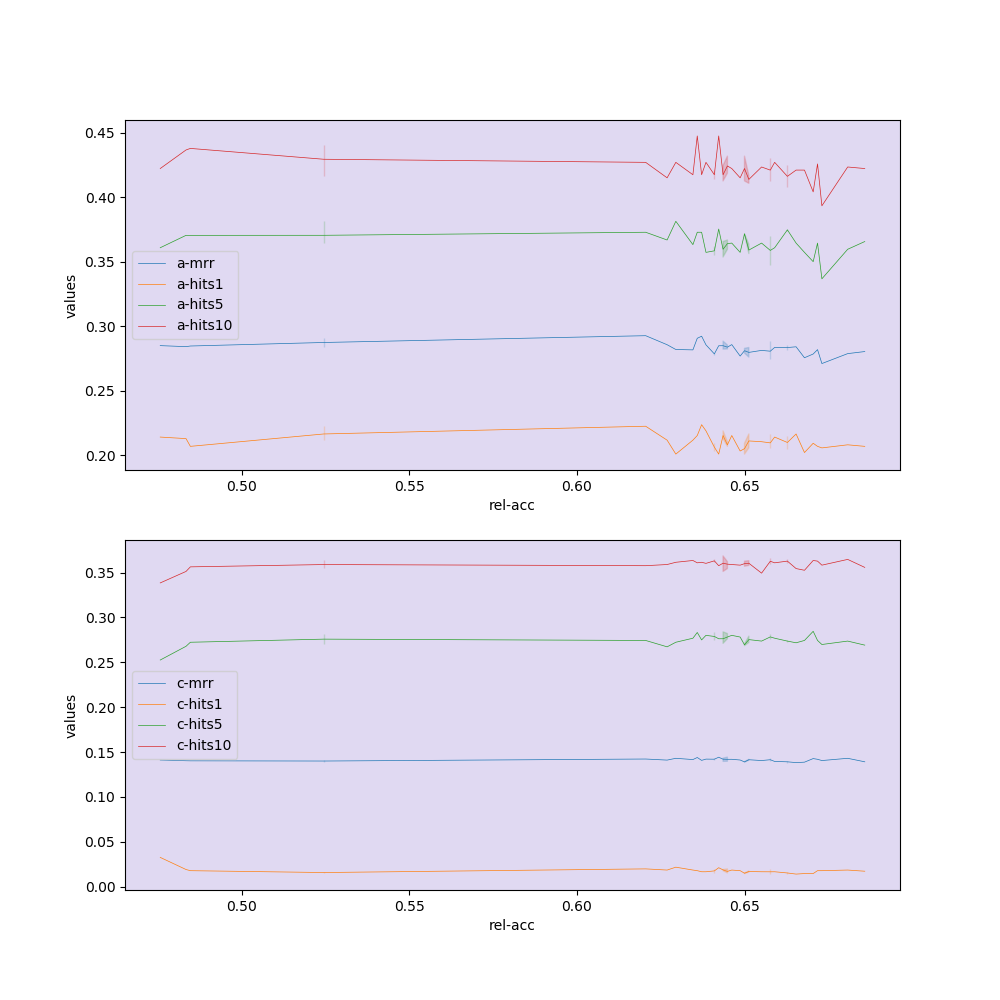
\includegraphics[scale=0.5]{0623/iptranse_C_S_V7_0621_lineplot_metrics.png}
    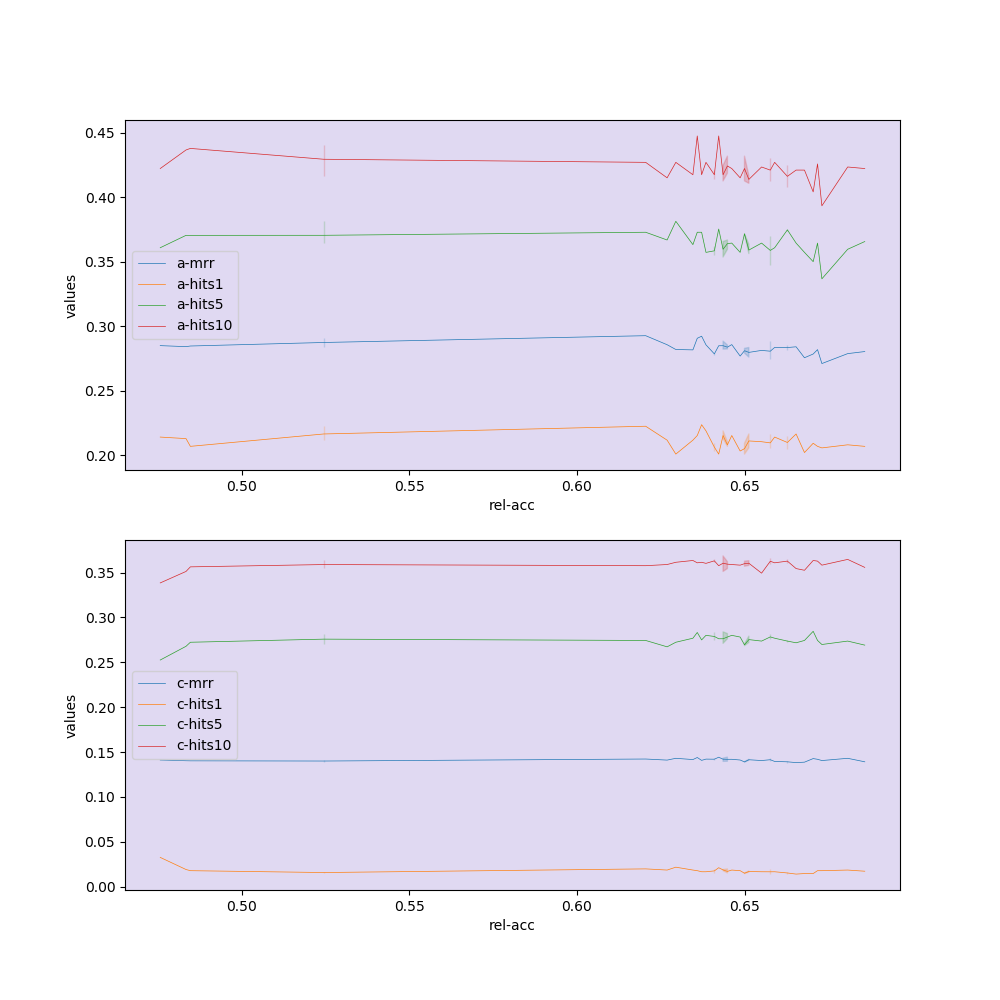
\includegraphics[width=\linewidth]{0623/iptranse_C_S_V7_0621_lineplot_metrics.png}
    \caption{\label{fig:iptranse_C_S_V7_0621_lineplot_metrics} Correlations between rel-acc and other metrics. Embedding matrices and relations types are optimized with two optimizers. Parameters in relation classifier are updated at first 100 epoches and then updated every 30 epoches in the remaining 900 epoches. Embedding matrices are updated at every epoch. The vibration is reduced compared with Figure~\ref{fig:iptranse_C_S_V7_0621_lineplot_metrics} and also the values of other metrics increased slightly. However, the average relaiton accuracy also dropped from 0.80 to 0.65 (underfitting). So in the next section, I tried to use less dropout rate and increase the learning rate and the hidden dimensions of relation classifier.}
\end{figure}
\clearpage

\section{Train 34 relation types}

Using similar startegy described as above. I run the model on the dataset with 34 types relations. Results are shown in Figure~\ref{tab:asynchronously_training_results}.
We can see the good news is the the overfitting problem is solved and the balance between rel-acc and other metrics is decent. When increasing the rel\_hidden\_dim from 100 to 500, the rel-acc also increases. 

One problem I observed from Figure~\ref{fig:asynchronously_training_results_curves} is that the vibrations of these loss curves are very strong (see the backgrounds of three losses.) They are decreasing overall, but not very stable. This could suggest that the leraning rate is too large, I should try to lower it. However,  the curves of metrics (Figure~\ref{fig:asynchronously_metrics_results_curves}) show lowering the learning rate also cause the dropping of performances. May be I could use a large learning rate at the beginning and a small one in the later phase. 


\begin{figure}[!ht]
    \centering
    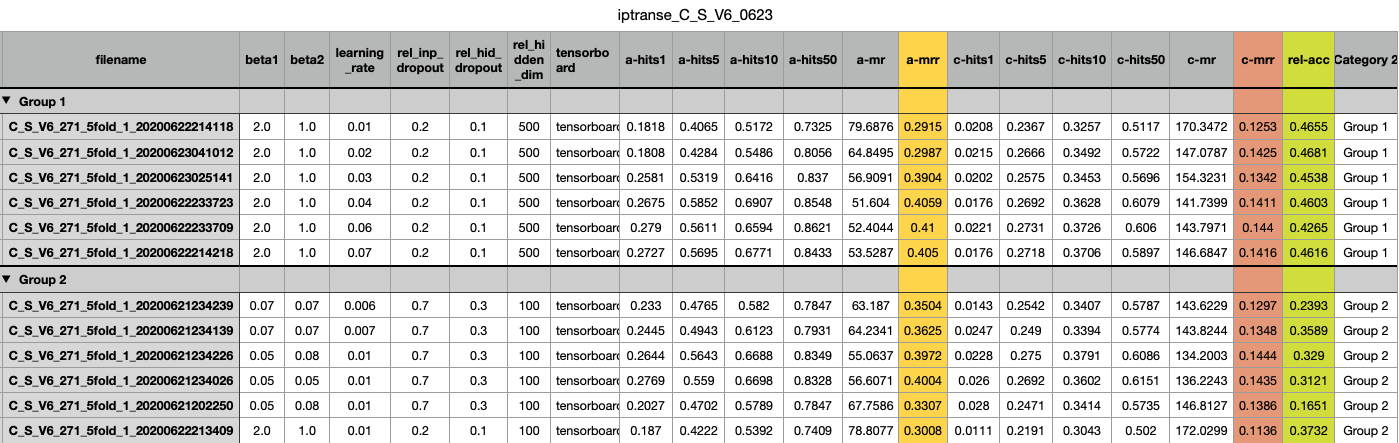
\includegraphics[width=\linewidth]{0623/C_S_V6_0623.png}
    \caption{\label{tab:asynchronously_training_results} Results for asynchronously training on 34 relation types. }
\end{figure}
\begin{figure}[!ht]
    \centering
    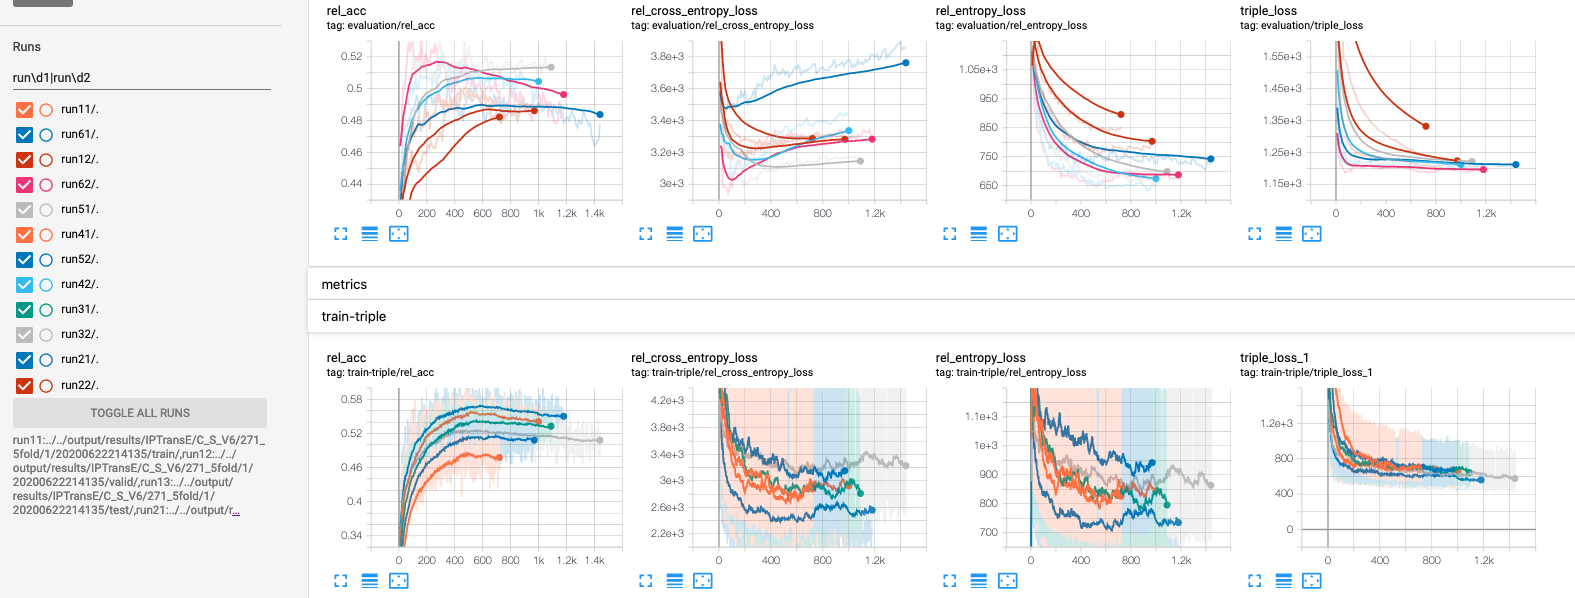
\includegraphics[width=\linewidth]{0623/C_S_V6_0623_learning_curves.png}
    \caption{\label{fig:asynchronously_training_results_curves} Learning curves for Group1 in Figure~\ref{tab:asynchronously_training_results} The top part is the evaluation curves, and the bottom is the training curves (run1* to run6* indicate the learning rate increases from 0.01 to 0.07. (0.05 is still running)).}
\end{figure}
\begin{figure}[H]
    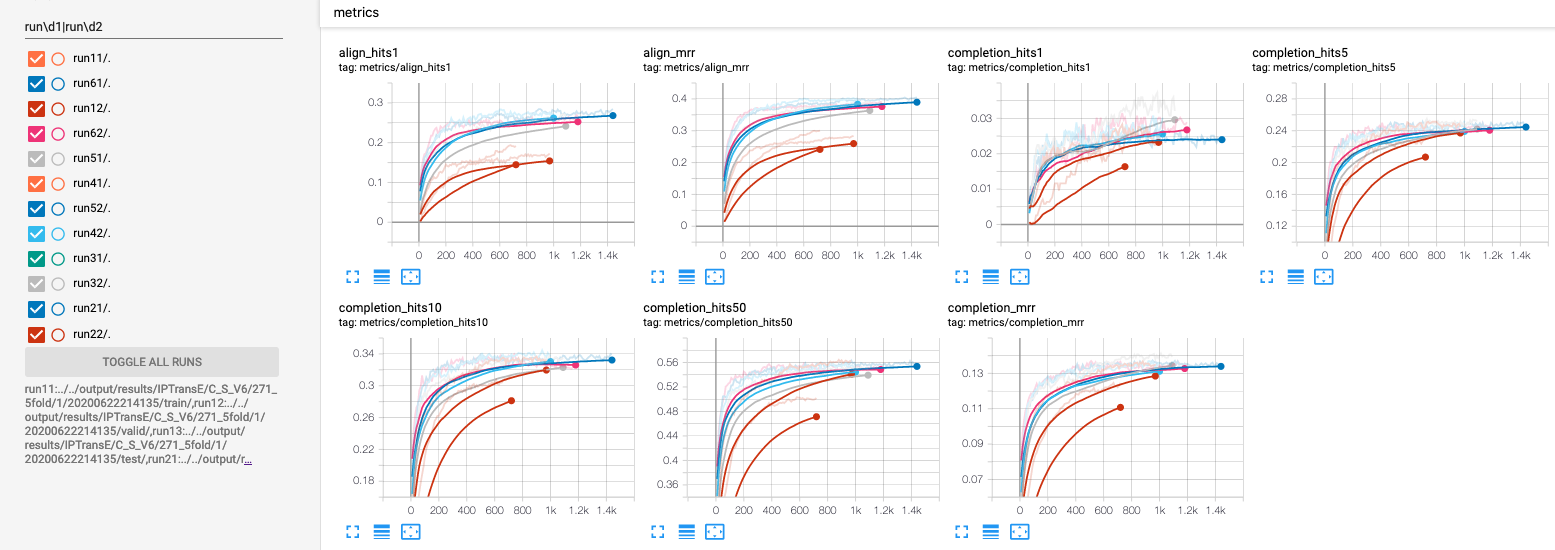
\includegraphics[width=\linewidth]{0623/C_S_V6_0623_metrics_curves.png}
    \caption{\label{fig:asynchronously_metrics_results_curves}  Curves of evaluation metrics for Group1 results in Figure~\ref{tab:asynchronously_training_results} }
\end{figure}

\section{Meeting Notes}


To do list 
\begin{enumerate}
    \item Observe the model outputs on rank, completion, relaiton classification task.
    \begin{enumerate}
        \item Case study: observe head, relation, and tail predictions 
        \item Relation classification confidence measure
        \item Alignment rank confidence measure
        \item Completion rank confidence measure
        \item Visualize the relation labelled SWOW graph. 
    \end{enumerate}
\end{enumerate}

\noindent Possible future directions: Expand to multilingual commonsense knowledge graphs alignment or completion. Becauae both ConceptNet and SWOW has multiple languages version.

\begin{comment}
beta1s=(0.05 0.05 0.05 0.05 0.05 0.05 0.05 0.05) 
beta2s=(0.05 0.08 0.08 0.08 0.08 0.08 0.08 0.05) 
lrs=(0.01 0.007 0.006 0.005 0.004 0.003 0.002 0.001

beta1s=(0.07 0.07 0.07 0.07 0.07 0.07 0.07 0.07) 
beta2s=(0.07 0.07 0.07 0.07 0.07 0.07 0.07 0.07) 
lrs=(0.01 0.007 0.006 0.005 0.004 0.003 0.002 0.001)

tensorboard --logdir=run11:"../../output/results/IPTransE/C_S_V6/271_5fold/1/20200622214135/train/",run12:"../../output/results/IPTransE/C_S_V6/271_5fold/1/20200622214135/valid/",run13:"../../output/results/IPTransE/C_S_V6/271_5fold/1/20200622214135/test/",run21:"../../output/results/IPTransE/C_S_V6/271_5fold/1/20200623041025/train/",run22:"../../output/results/IPTransE/C_S_V6/271_5fold/1/20200623041025/valid/",run23:"../../output/results/IPTransE/C_S_V6/271_5fold/1/20200623041025/test/",run31:"../../output/results/IPTransE/C_S_V6/271_5fold/1/20200623025154/train/",run32:"../../output/results/IPTransE/C_S_V6/271_5fold/1/20200623025154/valid/",run33:"../../output/results/IPTransE/C_S_V6/271_5fold/1/20200623025154/test/",run41:"../../output/results/IPTransE/C_S_V6/271_5fold/1/20200622233738/train/",run42:"../../output/results/IPTransE/C_S_V6/271_5fold/1/20200622233738/valid/",run43:"../../output/results/IPTransE/C_S_V6/271_5fold/1/20200622233738/test/",run51:"../../output/results/IPTransE/C_S_V6/271_5fold/1/20200623072050/train/",run52:"../../output/results/IPTransE/C_S_V6/271_5fold/1/20200623072050/valid/",run53:"../../output/results/IPTransE/C_S_V6/271_5fold/1/20200623072050/test/",run61:"../../output/results/IPTransE/C_S_V6/271_5fold/1/20200622233723/train/",run62:"../../output/results/IPTransE/C_S_V6/271_5fold/1/20200622233723/valid/",run63:"../../output/results/IPTransE/C_S_V6/271_5fold/1/20200622233723/test/",run71:"../../output/results/IPTransE/C_S_V6/271_5fold/1/20200622214236/train/",run72:"../../output/results/IPTransE/C_S_V6/271_5fold/1/20200622214236/valid/",run73:"../../output/results/IPTransE/C_S_V6/271_5fold/1/20200622214236/test/",run81:"../../output/results/IPTransE/C_S_V6/271_5fold/1/20200623061933/train/",run82:"../../output/results/IPTransE/C_S_V6/271_5fold/1/20200623061933/valid/",run83:"../../output/results/IPTransE/C_S_V6/271_5fold/1/20200623061933/test/"
\end{comment}
\begin{comment}
\chapter{2020-06-16}
\textbf{Checklist}
\begin{enumerate}
    \item \faCheckSquareO Performance gap between valid and test. \\ 
    Give a better explanation about why alignment results on test is still better than valid. (The candidates for valid is half less than the test, but the valid mrr is still lower than the test.)

    \item \faTimesCircleO Relation classification is still overfitting.
    %\begin{enumerate}[label*=\arabic*.]
    \begin{enumerate}
        \item \faCheckSquareO Try applying a dropout to the output of hidden layer, not only just the input of hidden layer.
        \item \faCheckSquareO Try adding more hidden layers.
        \item \faCheckSquareO Try lowering the ratio and scale of $\beta_1$ for relation cross entropy loss.  
    \end{enumerate}

    \item KG completion evaluation 
     \begin{enumerate}
        \item \faCheckSquareO Check the code for evaluating on KG completion
        \item \faCheckSquareO Use the overall loss for early stopping instead of only the hits1 on alignment
        \item \faCheckSquareO Figure out why completion results (hits@N, mrr, mr) are pretty bad, why it's much worse than alignment (why completion task is harder than alignemnt task).
    \end{enumerate}

    \item \faCheckSquareO Make sure the baseline is all good. Compare the model with or without relation calssifier.
    \item Draw the heatmap for $\beta_1$ and $\beta_2$ with rel\_acc and mrr.
    \item \faCheckSquareO Make sure the test data is not used for training.
    \item Pre-train the relation-classifier and then freeze it to train other parts of models. 
    \item Design better negative sampling strategies. 
\end{enumerate}

\section{Overfitting on relation classification}
Now the relation classifier is a three layers of FNN. 
When I tried to dropout the inputs of the first and second layer, it indeed can prevent the overfitting when the dropout rate is set to 0.8 or 0.9. But too much dropout caused the the 'NAN' incidently and interrupt the training. This is because the relation types are accidently all set to zero.
So I have to reduce the dropout rate, and then the overfitting on appeared again. (Still need to try some other ways.)

\section{Performance Gap between Valid and Test}
The performance (mrr and hits) gap on alignment task between the valid set and test set is caused by the sampling order. \textbf{When first created them, I sampled the test set first, and then sampled the valid set.} The sampling process tends to sample the entities with higher frequency, which caused the frequencies in valid set is much higher than test set. Entities with higher frequency are easier for model to learn a better embedding, and thus leads to higher alignemnt performance. 
For entities on valid and test, I visualized them frequency distribution in both the overlap\_subset, ConceptNet and SWOW. 


\begin{figure}[!ht]
    \centering
    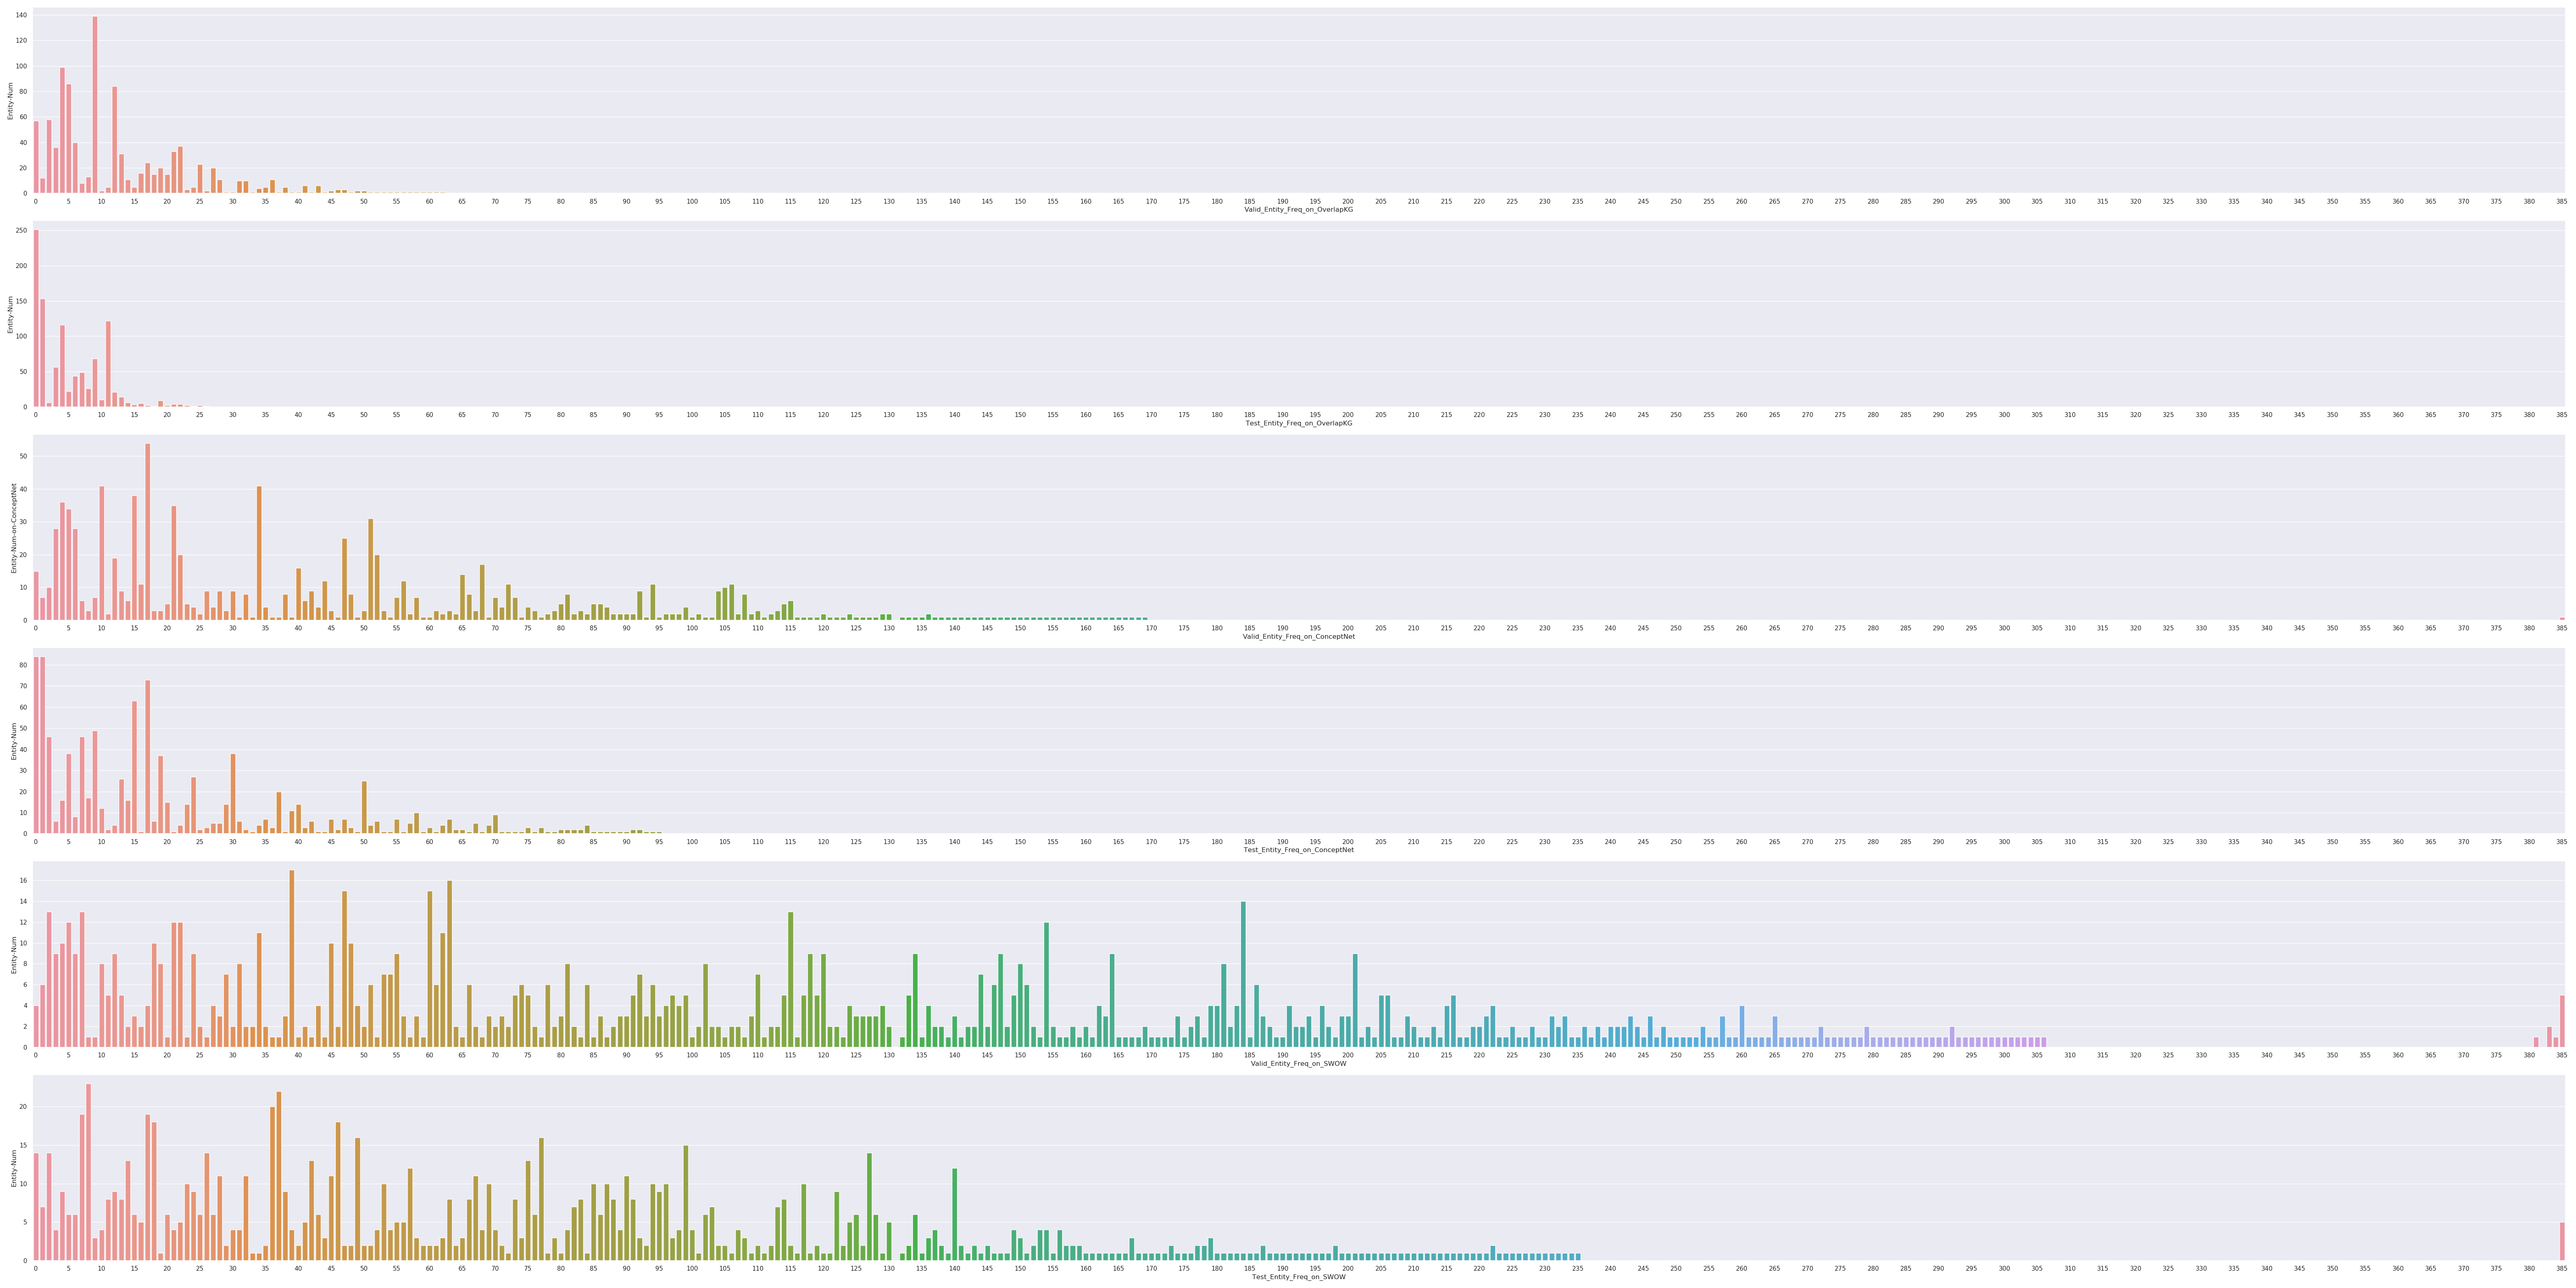
\includegraphics[width=\textwidth]{images/0616/C_S_V4_valid_test_ent_freq_distributions.png}
    \caption{\label{fig:biased_valid} Biased to valid: sample valid first. The odd row for valid and the even row is for test.}
\end{figure}
\begin{figure}[!ht]
    \centering
    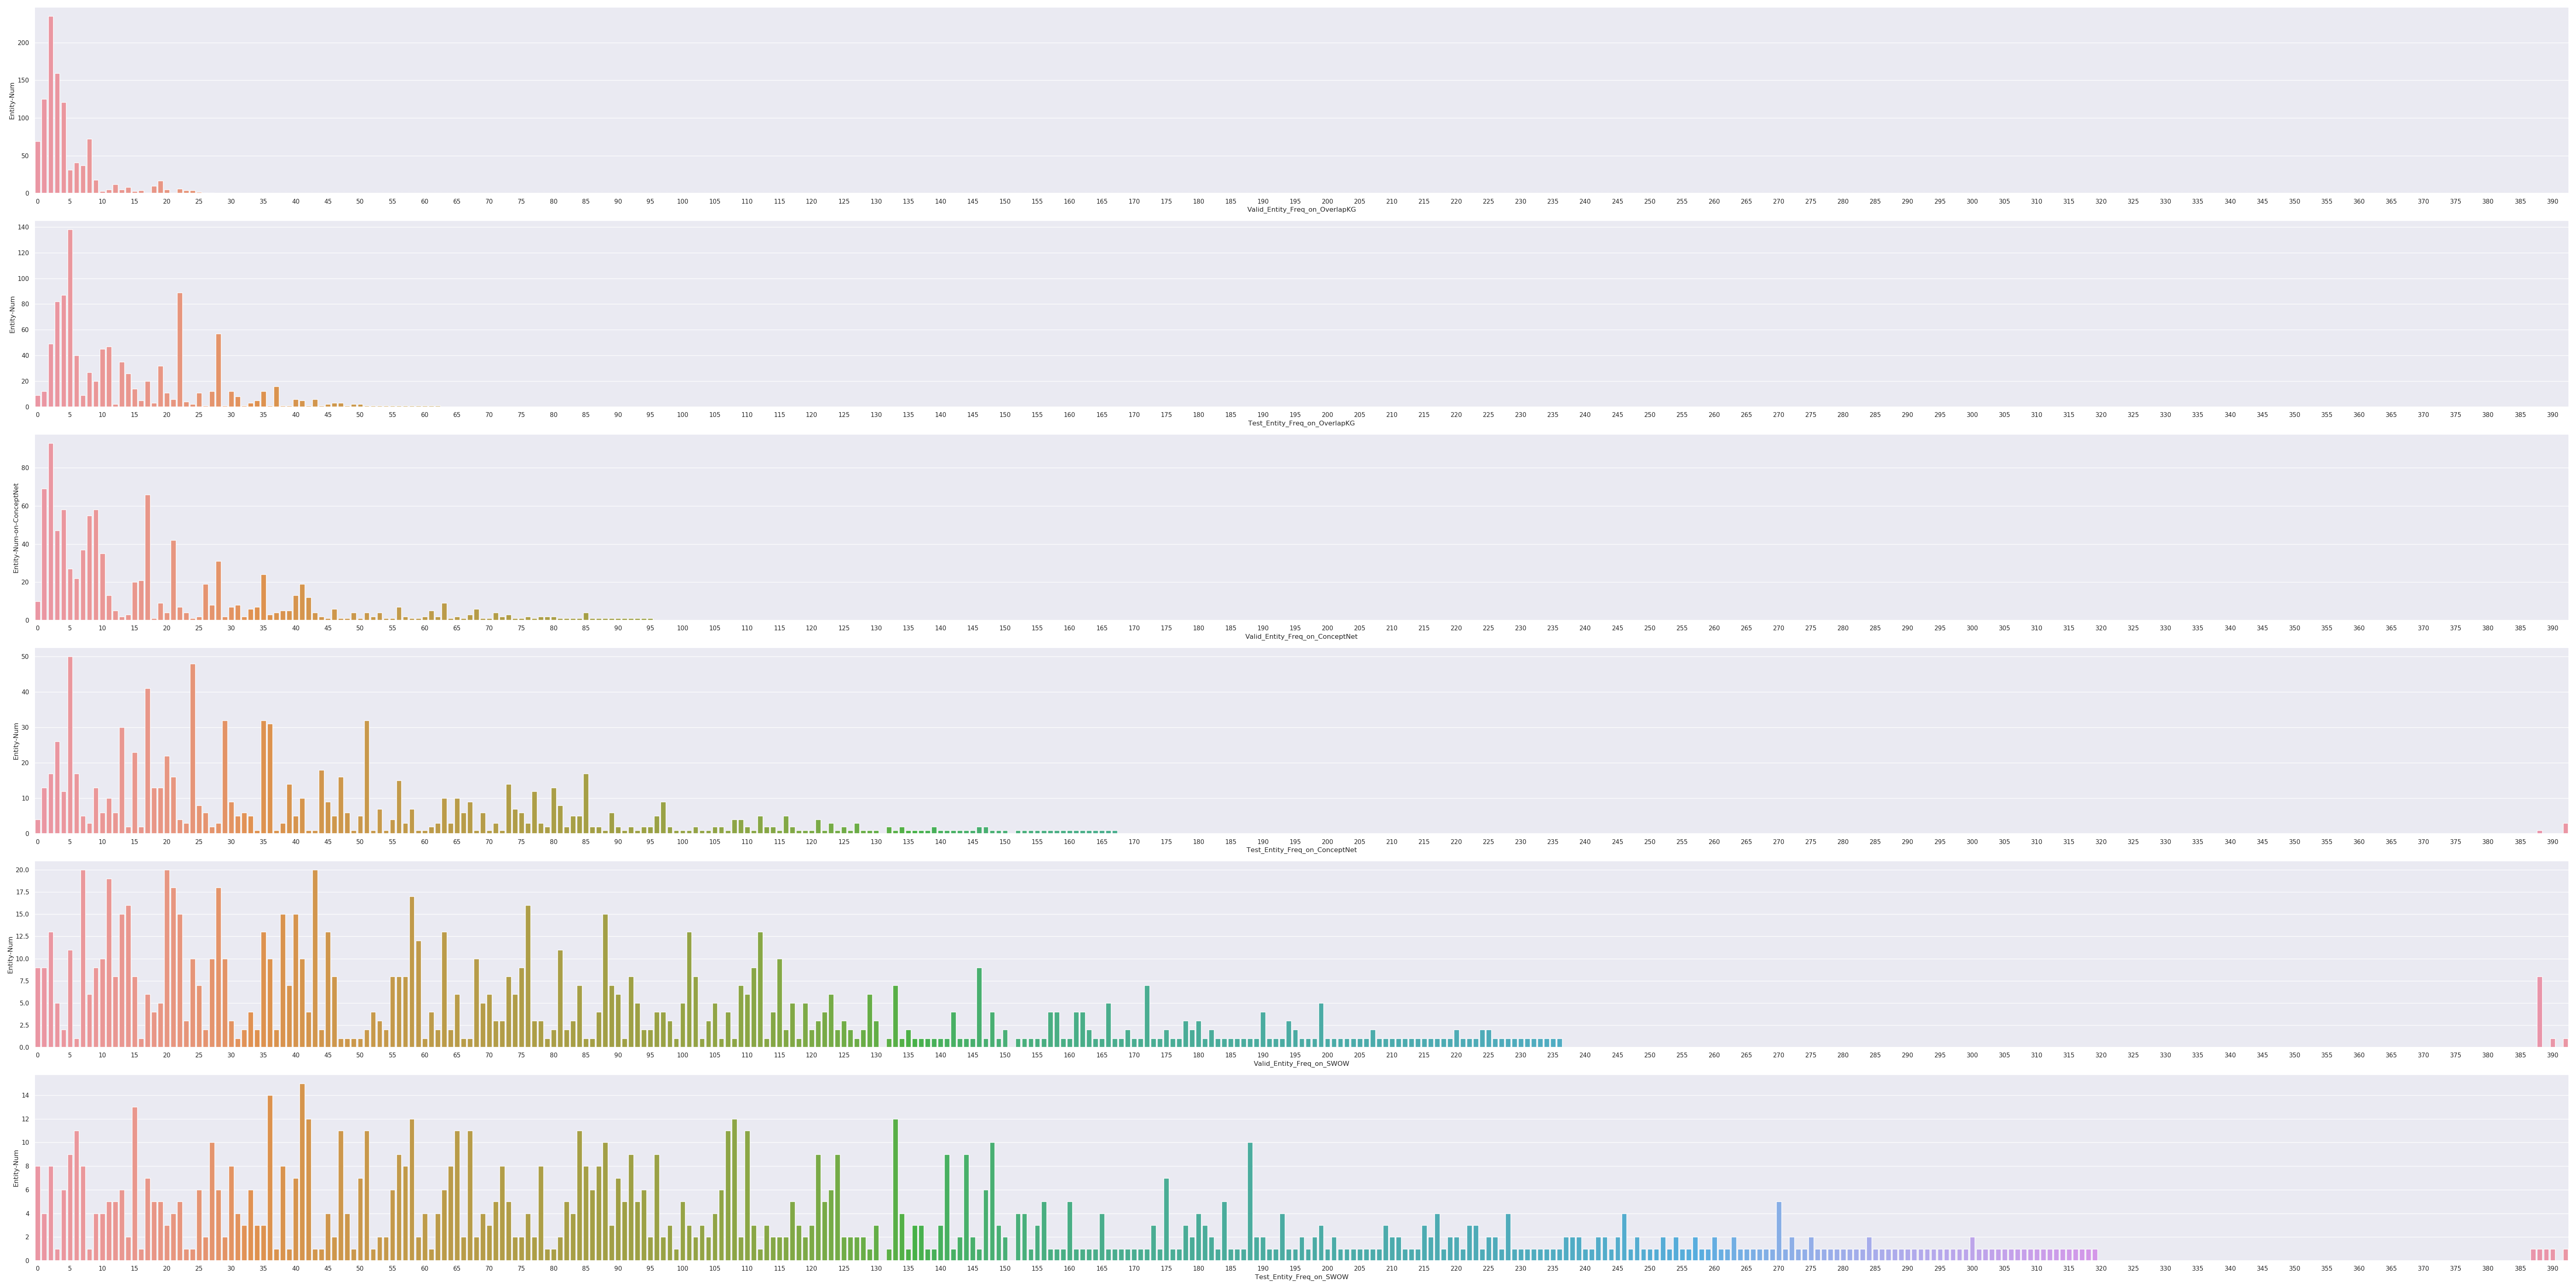
\includegraphics[width=\textwidth]{images/0616/C_S_V5_valid_test_ent_freq_distributions.png}
    \caption{\label{fig:biased_test} Biased to test: sample test first. The odd row for valid and the even row is for test.}
\end{figure}
\begin{figure}[!ht]
    \centering
    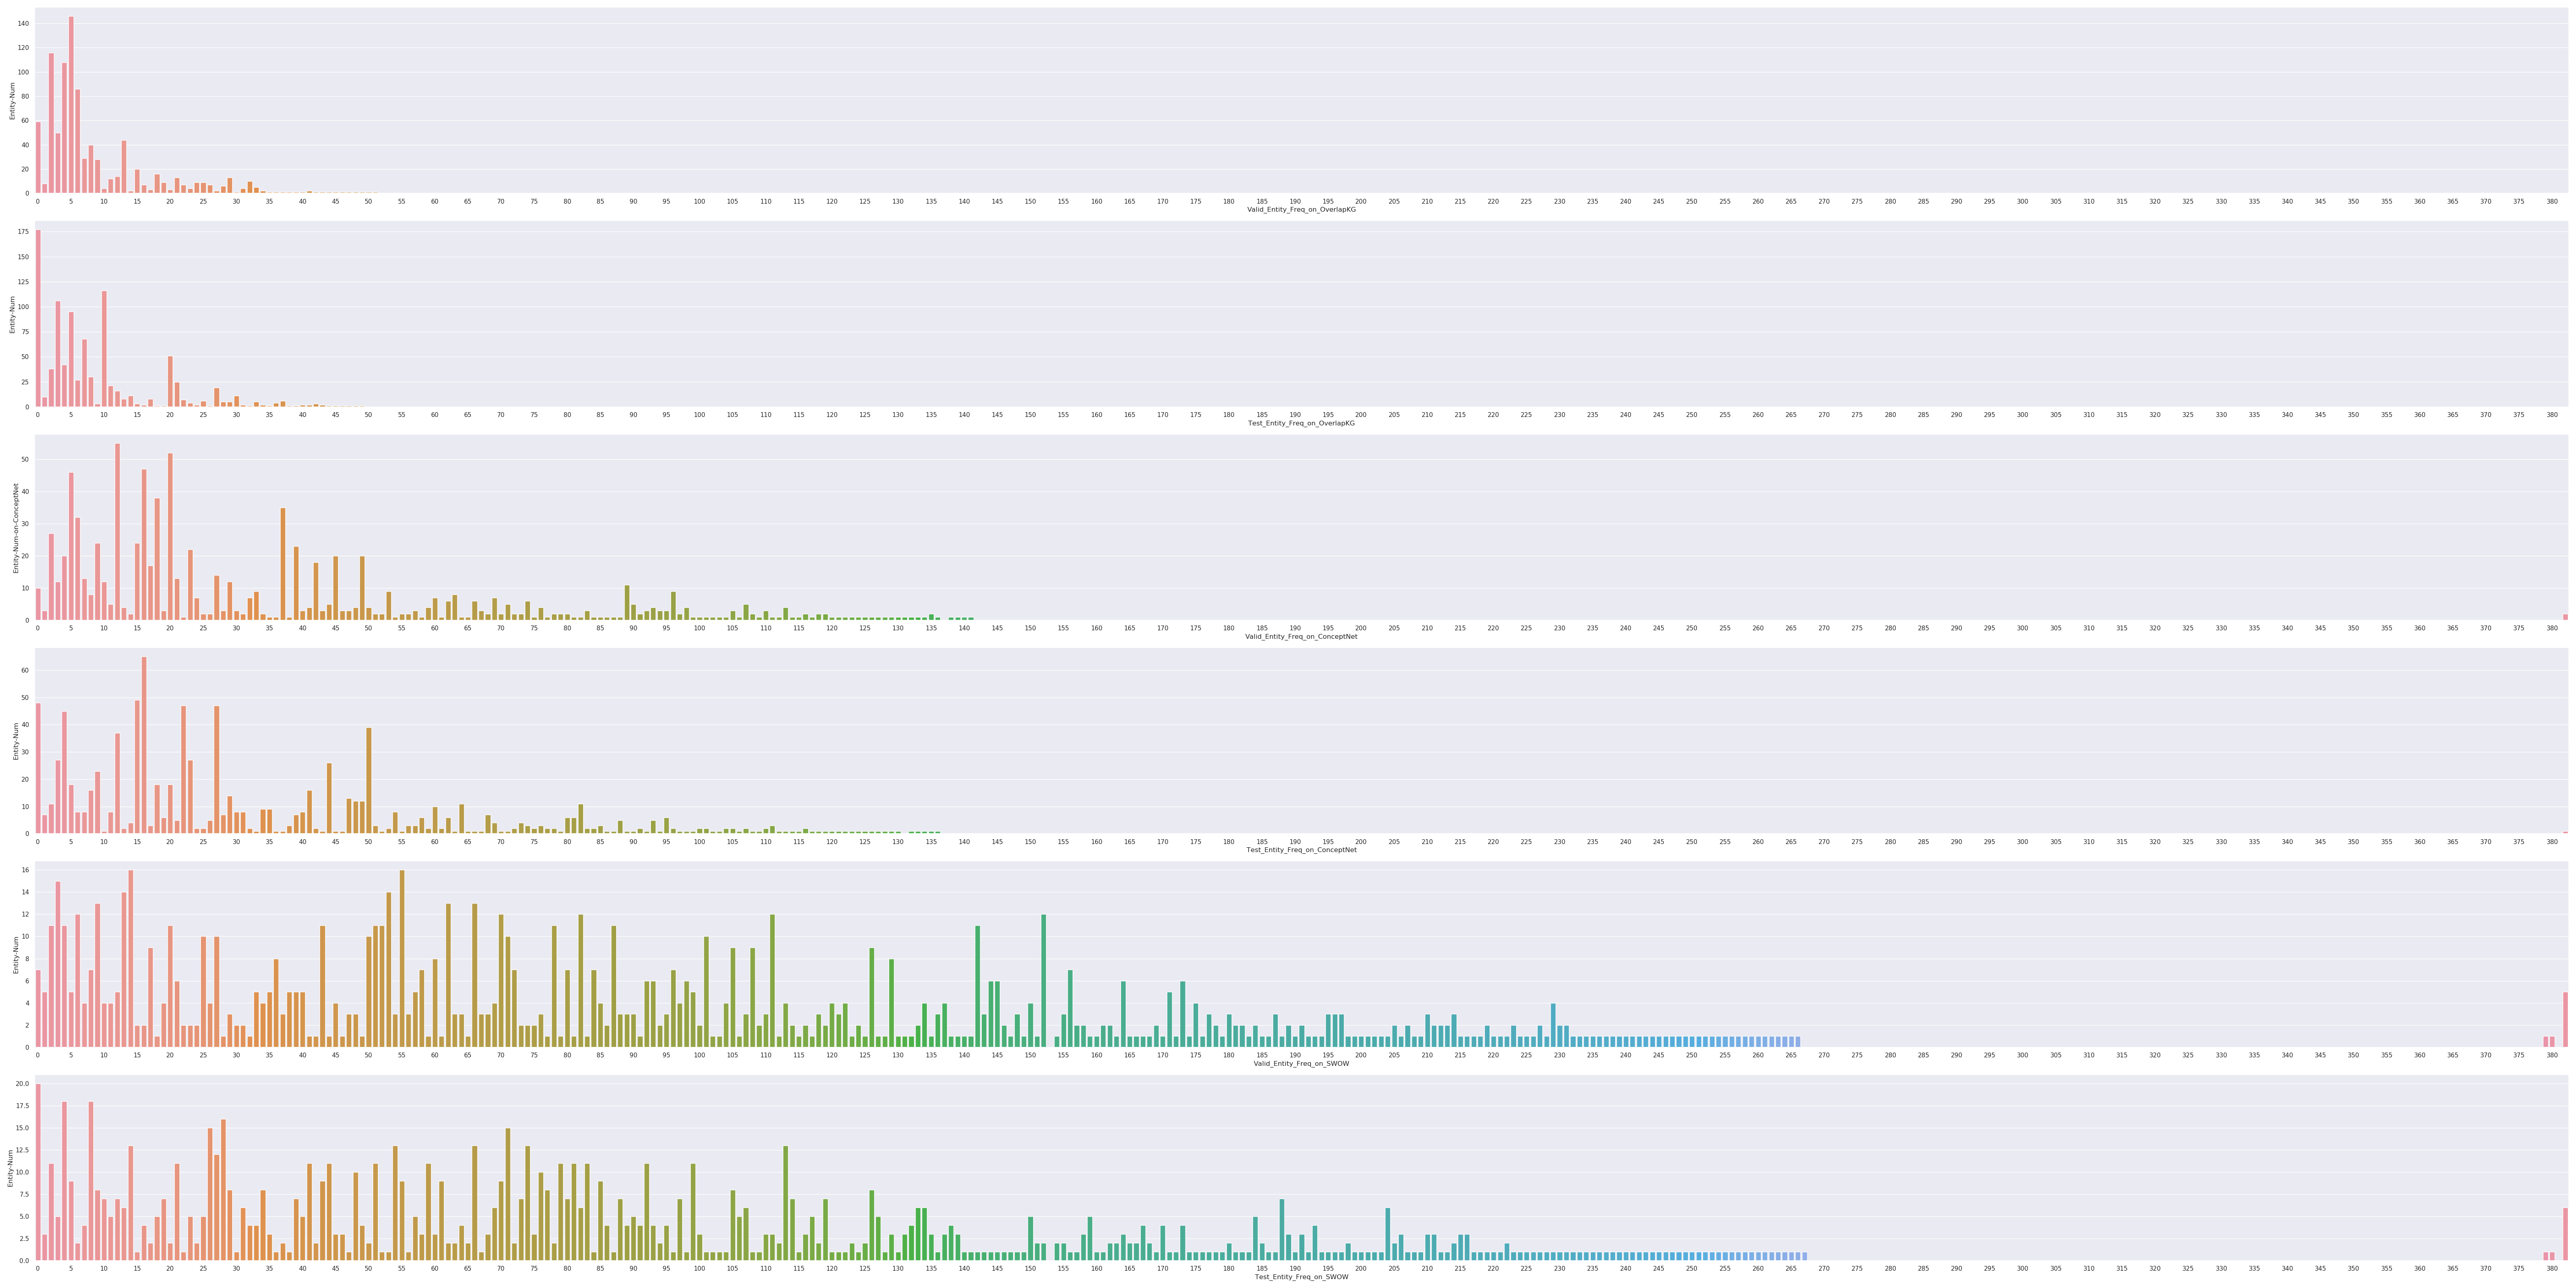
\includegraphics[width=\textwidth]{images/0616/C_S_V6_valid_test_ent_freq_distributions.png}
    \label{fig:unbiased_valid_test_ent_freq_distributions}
    \caption{Bias reduced sample: sample valid and test iteratively with a number of min-batch. The odd row for valid and the even row is for test.}
\end{figure}
By comparing the three frequency distributions, we can see that entities sampled first have higher frequency and infer higher frequency entities leads to better evaluation performance.  
I also compared the alignemnt-mrr curves for valid and test during trining process and testified this hypothesis (see figure ~\ref{fig:comparision_of_different_sample_valid_test_order}).

%The Figure~\ref{fig:biased_valid}, 
Figure~\ref{fig:biased_test}, and Figure~\ref{fig:unbiased_valid_test_ent_freq_distributions} show the frequency distribution for entities in the valid and test. 
The x-axis is the frequency of a entity, the y-axis is the entity num with correspoing frequency in the test/valid set. Figure~\ref{fig:biased_valid} is the frequency distributions of sampling valid first and Figure~\ref{fig:unbiased_valid_test_ent_freq_distributions} is the frequency distributions by sampling valid and test iteratively with a min-batch sample size to minimize the gap between them. Also, to control the influence of total rank candidates number, I tried to keep the overall entity number in the valid and test to be close (see Table~\ref{tab:statistics_two_versions_valid_test}).

\begin{figure}[!ht]
    \centering
    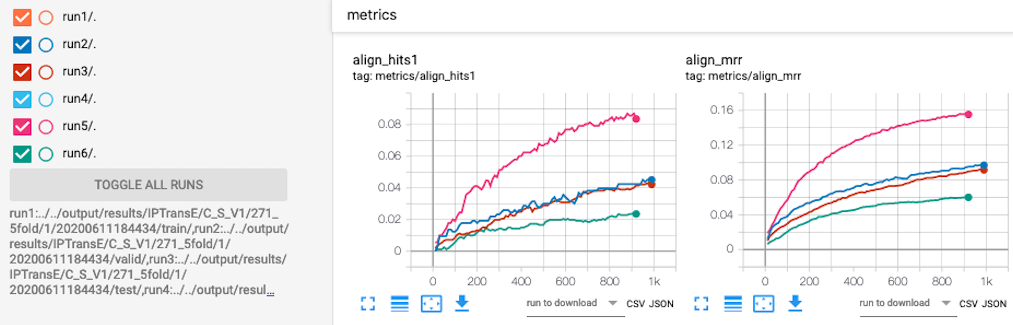
\includegraphics[width=\textwidth]{images/0616/comparision_of_different_sample_valid_test_order.png}
    \caption{\label{fig:comparision_of_different_sample_valid_test_order} Comparsion of biased and unbiased sample. The pink and green curves are the biased valid and test (sample valid first). The blue and orange curves are the unbiased valid and test. The gap between the unbiased are much smaller. }
\end{figure}

\begin{table}[H]
    \centering
    \begin{tabular}{cccc}
        \hline
        Version &Dataset & \#Triples &\#Entities \\
        \hline
        previous & valid & 565	&742\\
        previous & test & 1,236	&1,521\\
        \hline
        current & valid & 778	& 914\\
        current & test & 769	& 957\\
        \hline
    \end{tabular}
    \caption{\label{tab:statistics_two_versions_valid_test} Statistics for two different versions of valid and test.}
    
\end{table}

\clearpage
\section{Experimental Results}
Our hypothesis is joinly train ConceptNet and SWOW could possibly learn a knowledge shared embedding matrix for them. 

\subsection{Baselines}

\begin{figure}[!ht]
    \centering
    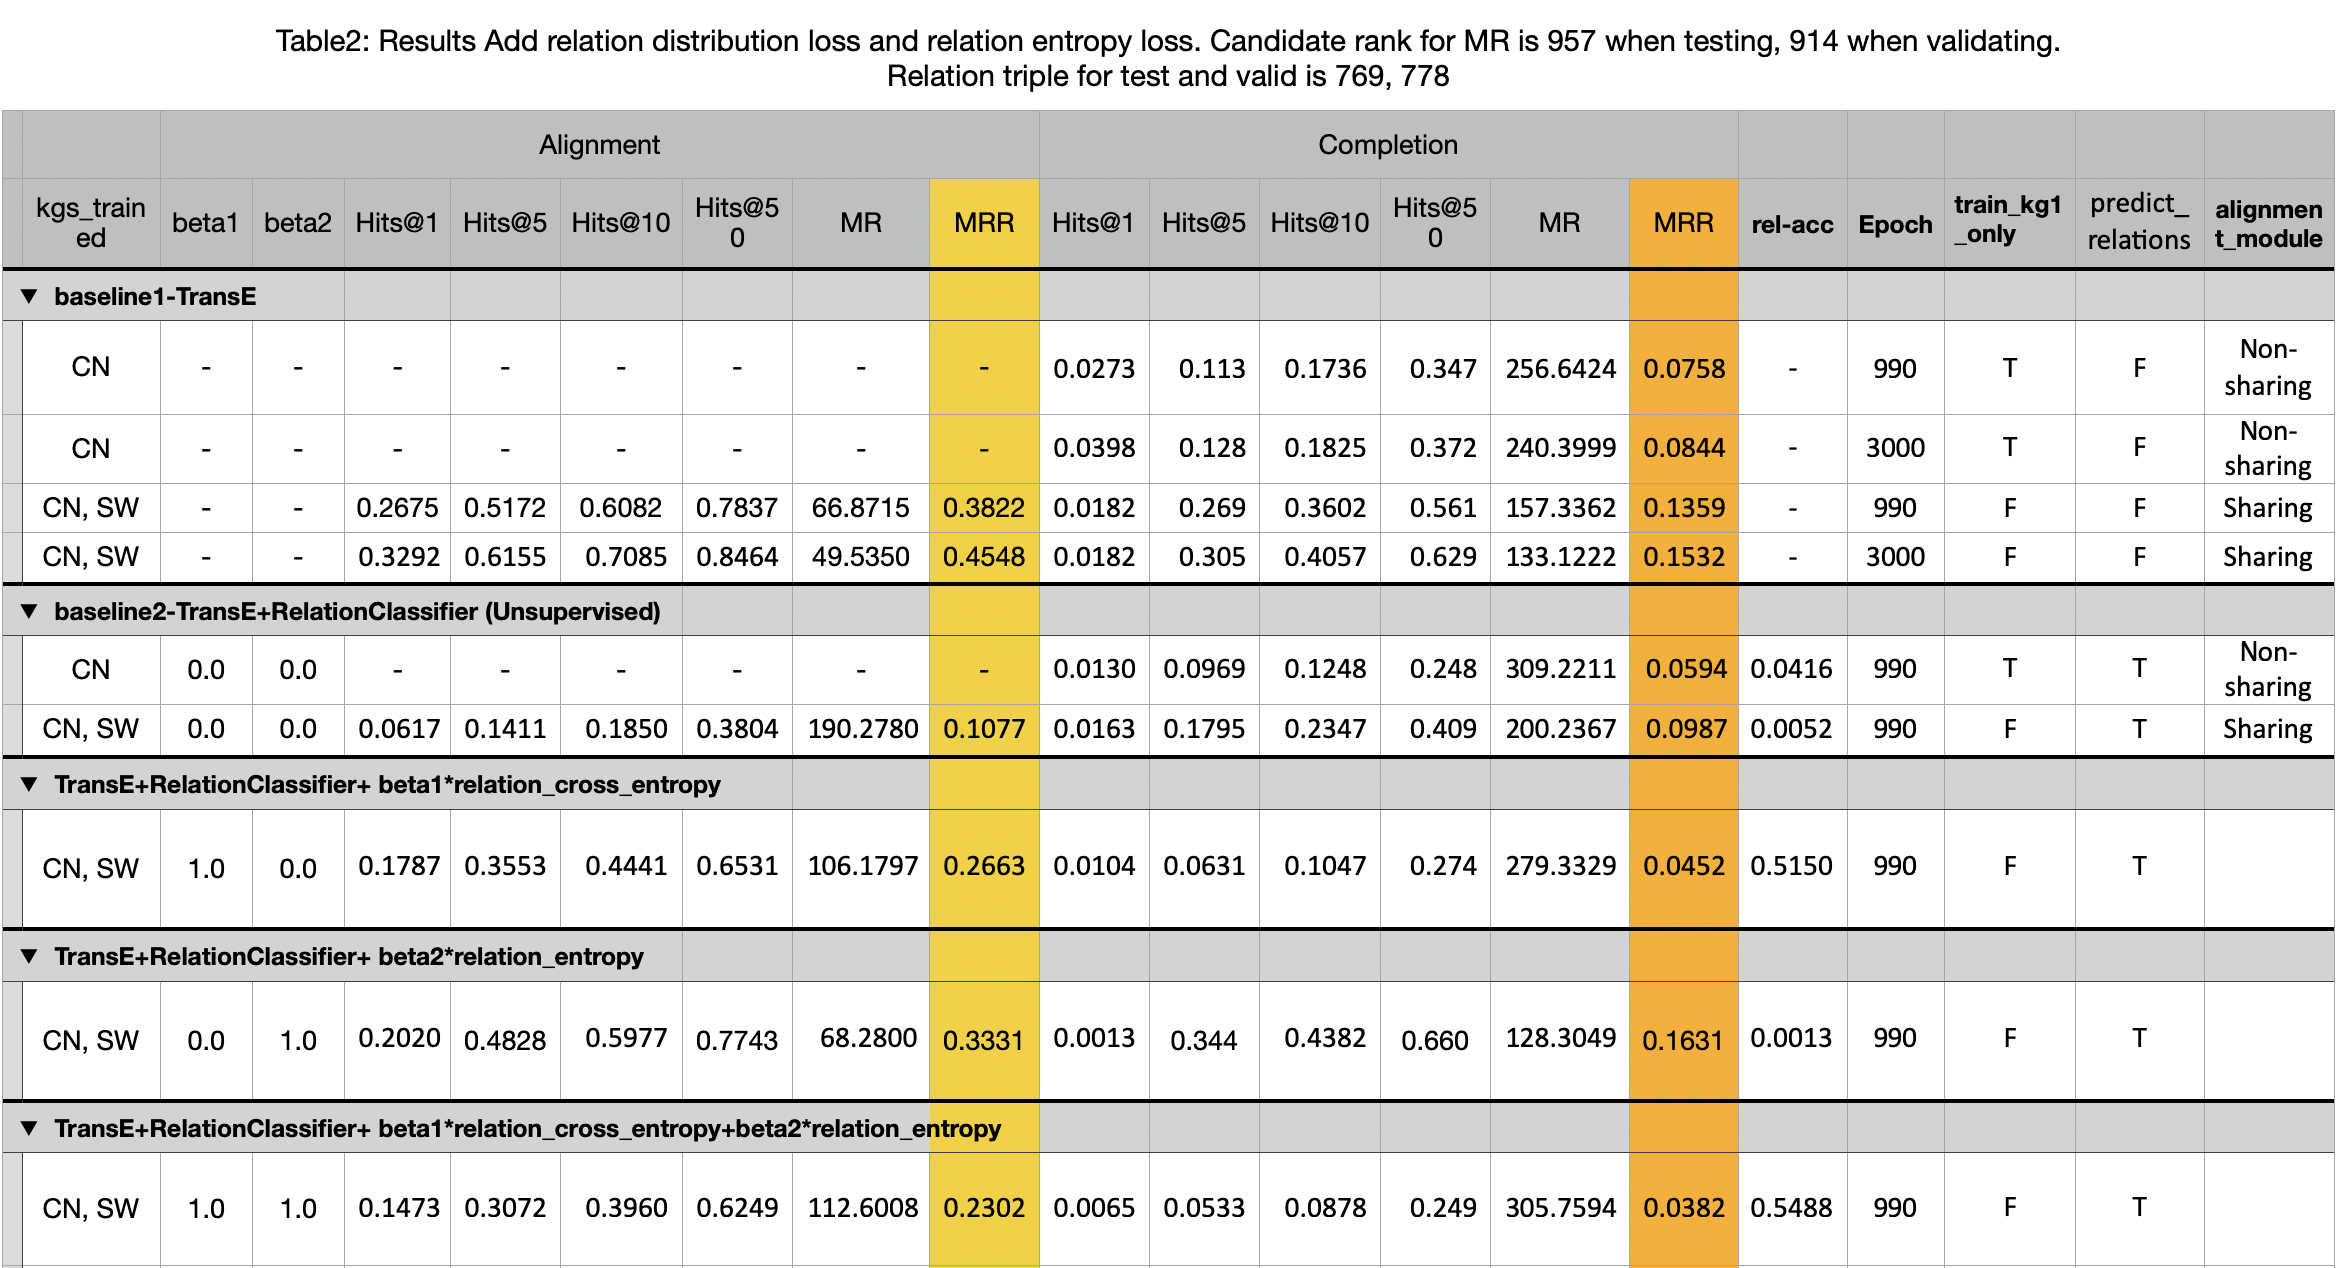
\includegraphics[width=\textwidth]{0616/baseline_results.png}
    \caption{Baseline Results}
    \label{tab:baseline_results}
\end{figure}
Observations from Figrue~\ref{tab:baseline_results}:
\begin{enumerate}
    \item Compare the results of baseline1-TransE, we can see the joinly training of ConceptNet and SWOW indeed help the completion on their overlap triples. Also, the MRR is increasing with the increase of trainig time when jointly train them. 
    \item When adding the relation calssifier into the model without relation type supervision, the performances dropped a lot, especially on the alignemnt task. This may suggest that the relation type is important for the learning of entity embeddings. 
    \item When the cross entropy loss is added on TransE loss, the accuracy of relation classification raises to 0.5150. The alignemnt MRR goes up but the completion MRR keeps going down.  
    \item When the entropy loss is added to constrain the relation distributions, the alignemnt MRR go back to the same level as the baseline1-TransE, and the completion MRR achieves even higher score than baseline1-TransE. Also, with supervison, the relation classification accuracy declined. This result is very interesting. It shows the model can learn good entity embeddings even when the relation types are not correctly predicted. This is contrary to our intuitive. Our intuition is when model gives better relation predictions, it'll give better results on alignment and completion tasks.
\end{enumerate}

\clearpage
\subsection{Correlations between beta1,beta2 and metrics}
%\textbf{Correlations between $\beta_1$, $\beta_2$ and metrics}

\begin{figure}[!ht]
    \centering
    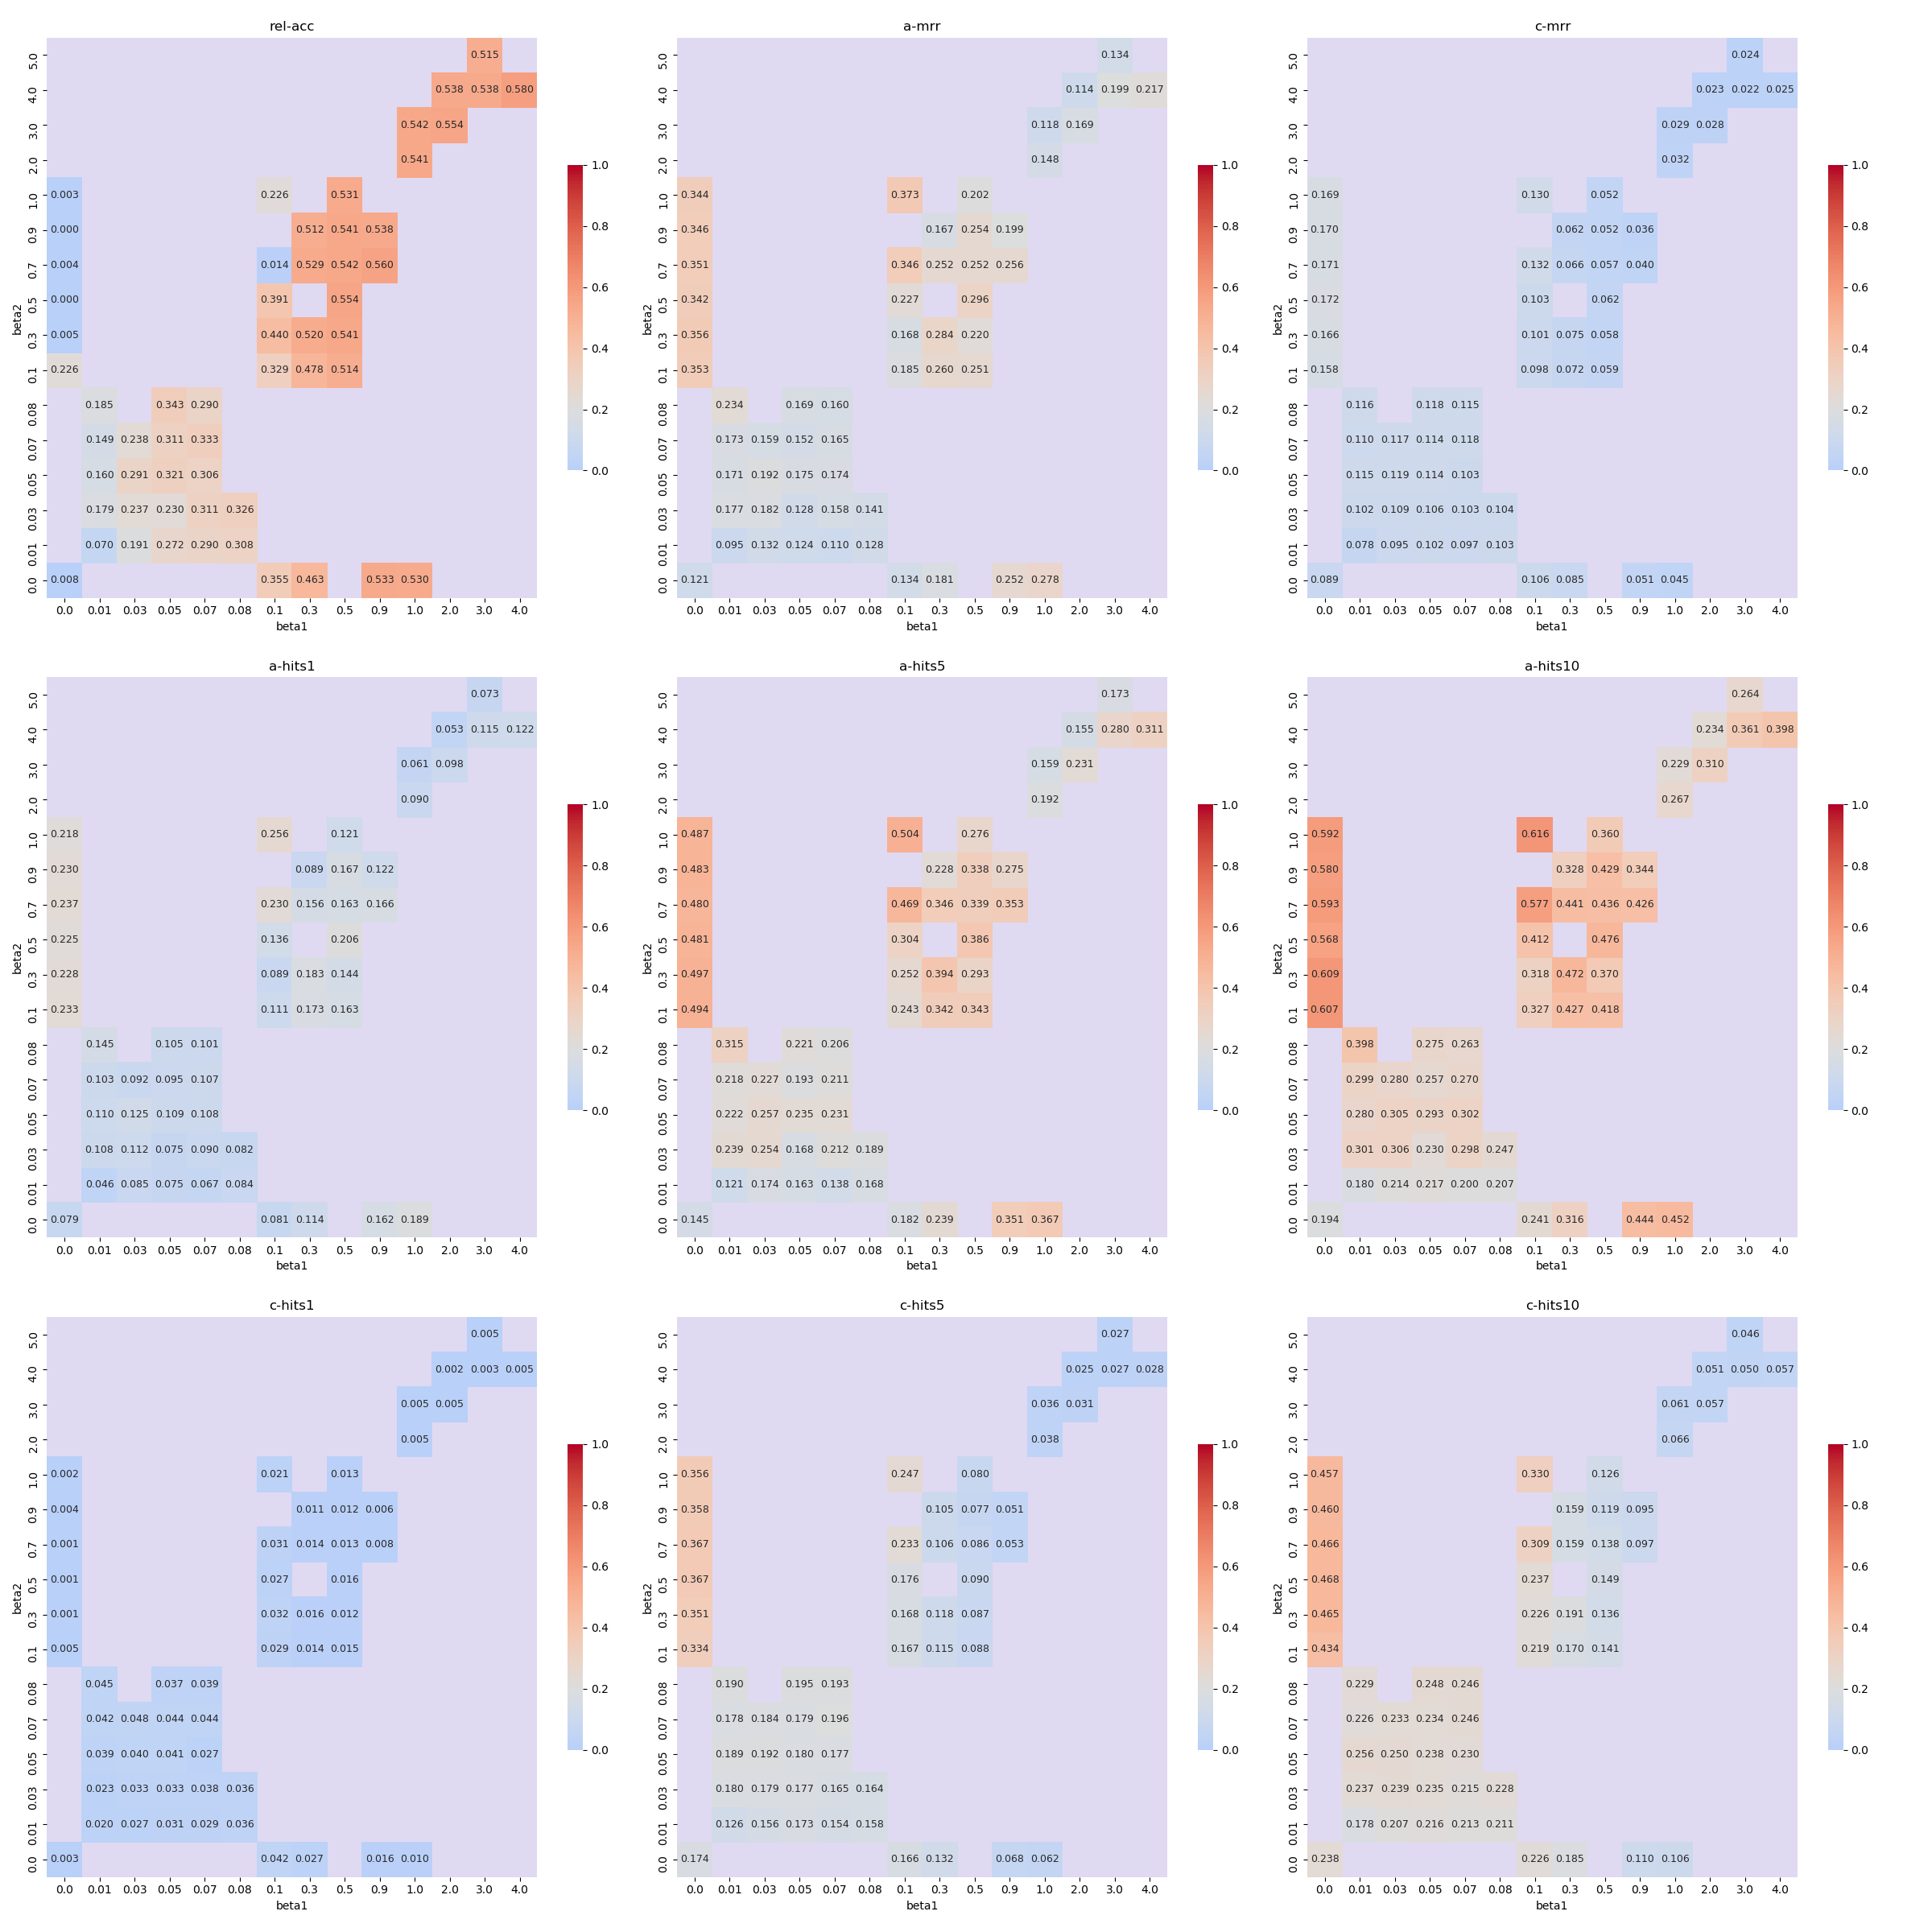
\includegraphics[width=\textwidth]{0616/heatmap_metrics.png}
    \caption{Relations between $\beta_1$, $\beta_2$ and various evaluation metrics.}
    \label{fig:heatmap_metrics}
\end{figure}
From Figure~\ref{fig:heatmap_metrics} can be seen that when $\beta_1$ is around 0.1, all the metrics look normal. But when increasing the $\beta_1$, e.g., $\beta_1 = 0.3$, the c-mrr would fall into very small value. However, the rel-acc is better when the $\beta_1$ is larger. The balance between them still needs to explore.

\clearpage
\section{Meeting Notes}
\textbf{Long term to do list}
\begin{enumerate}
    \item Find smarter negative sampling strategies.
\end{enumerate}

\noindent\textbf{Next week to do list}
\begin{enumerate}
    \item \faCheckSquareO Figure out why `NAN' appears during training. \\
        A: the scores for some relation types are too small and caused the underflow when apply log function to them. A small number 1e-9 is added to the scores for numerical stable.
    \item Debug the relation classifier \\
    For now, when $\beta_1$ is increased, the relation prediction accuracy become higher, but the alignment and completion performances dropped.  Try to figure out why, the code problem or the idea problem?
    Try to make the model and task to be simple to debug the relation classifier. 
    \begin{enumerate}
        \item \faCheckSquareO Lea: ``I was suggesting to come up with simpler variants (a toy data set, or limiting labels to only 2 classes) and see if your model behaves more meaningfully in these simplified scenarios... It may point you to issues with the implementation, or data set."
        \item Observe some prediction outputs for alignment rank, completion rank, and relation prediction (both training and valid). 
    \end{enumerate}
    
    \item Relation classification overfitting: try different training strategy to alleviate the problem. 
    \begin{enumerate}
        \item \faCheckSquareO Play with hyperparameters: lr, batch\_size, and training\_epoch. 
        \item \faCheckSquareO Pretrain the relation classifier.
        \item \faCheckSquareO Train the relation classifier every K ($K$ \textgreater $1$) iterations instead of every iteration. 
    \end{enumerate}

\end{enumerate}
papers lea has sent to me:
https://www.ijcai.org/Proceedings/2018/0581.pdf
https://www.ijcai.org/Proceedings/2019/0733.pdf


\chapter{2020-06-09}

\textbf{Checklist}
\begin{todolist}
    \item[\done] For valid sets:
        \begin{enumerate}
            \item Figure out why hits and mrr on valid set is much lower than test set. 
            \item Visualize training curves on valid set. (still haven't figure out) 
        \end{enumerate}
    \item Add evaluation on link prediction ($p(t|h,r)$) and triple classification (p(h,r,t) whether a triple exists).
    \item Add one more baseline: add the relation calssifier on TransE model and evaluate it. 
    \item Analysis on $\beta_1$ and $\beta_2$: 
    \begin{enumerate}
        \item Zoom in current $\beta_1$ (0-0.1) and $\beta_2$ (0.1-0.2) to see how they influce the MRR and the  REL\_ACC 
        \item Scale up the $\beta_1$ and $\beta_2$ to balance the scale range between $L_r$ and $L_p$ with $L_e$. (Because $L_e \approx 5*L_r$ and $L_e \approx 10*L_p$.) 
        \item Draw the correlation between $\beta_1$ and $\beta_2$ with the evaluation matrics. Observe how $\beta_1$ and $\beta_2$ influence the MRR or REL\_ACC.
    \end{enumerate}
    \item[\done] Print the confusion matrix for relation types to observe how model performs on each type.
    \item[\done] Apply dropout to model to tackle the overfitting problem of relaiton type accuracy.  
\end{todolist}


\clearpage
\section{Meeting Notes}
\begin{enumerate}
    \item Make sure the baseline is all good. Compare the model with or without relation calssifier.
    \item Relation classification is still overfitting.
    %\begin{enumerate}[label*=\arabic*.]
    \begin{enumerate}
        \item \faCheckSquareO Try applying a dropout to the output of hidden layer, not only just the input of hidden layer.
        \item \faCheckSquareO Try adding more hidden layers.
        \item Try lowering the ratio of $\beta_1$ for relation cross entropy loss.  
    \end{enumerate}
    \item Figure out why completion results (hits@N, mrr, mr) are pretty bad, why it's much worse than alignment (why completion task is harder than alignemnt task).
     \begin{enumerate}
        \item \faCheckSquareO Check the code for evaluating on KG completion
        \item \faCheckSquareO Use the overall loss for early stopping instead of only the hits1 on alignment
    \end{enumerate}
    \item Give a better explanation on why alignment results on test is still better than valid. (The candidates for valid is half less than the test, but the valid mrr is still lower than the test.)
    \item \faCheckSquareO Make sure the test data is not used for training.
    \item Draw the heatmap for $\beta_1$ and $\beta_2$ with rel\_acc and mrr.
    \item Pre-train the relation-classifier and then freeze it to train other parts of models. 
    \item Post my notes on slack before next monday night. (Thanks for Lea to remind me.)
\end{enumerate}
\graphicspath{{images/}}
\chapter{2020-06-02}
%\textbf{Checklist}
%\begin{todolist}
 %   \item[\done] Create test triples to evaluate learned relation embeddings (evaluate on relation type prediction).
%    \item[\done] Visualization1: Use tensorboard to draw the training curves for loss $L_e$, $L_r$, and $L_p$ on both train and dev. (note: train curves are drawn, dev curves of $L_r$ still have some problem (need to figure out why.)) 
%    \item[\done] Loss modification: Add entropy constraint for relation distribution $\alpha$. We hope the $\alpha$ to be inclined to one label, so the entropy of $\alpha$ should be small. 
%   \item[\done] Try learning a weight for the loss components
%    \item Visualization2: use TSNE to visualize $\alpha$. 
%    \item May try different kinds of negative sampling strategy, eg., sample nodes with similar degeree or similar frequency. 
%    \item Hidden units for relation classifier needs to be tuned. Now the $h \in R^{100}$, $t \in R^{100}$, $W \in R^{100}$
%\end{todolist}

%\section{Summary}
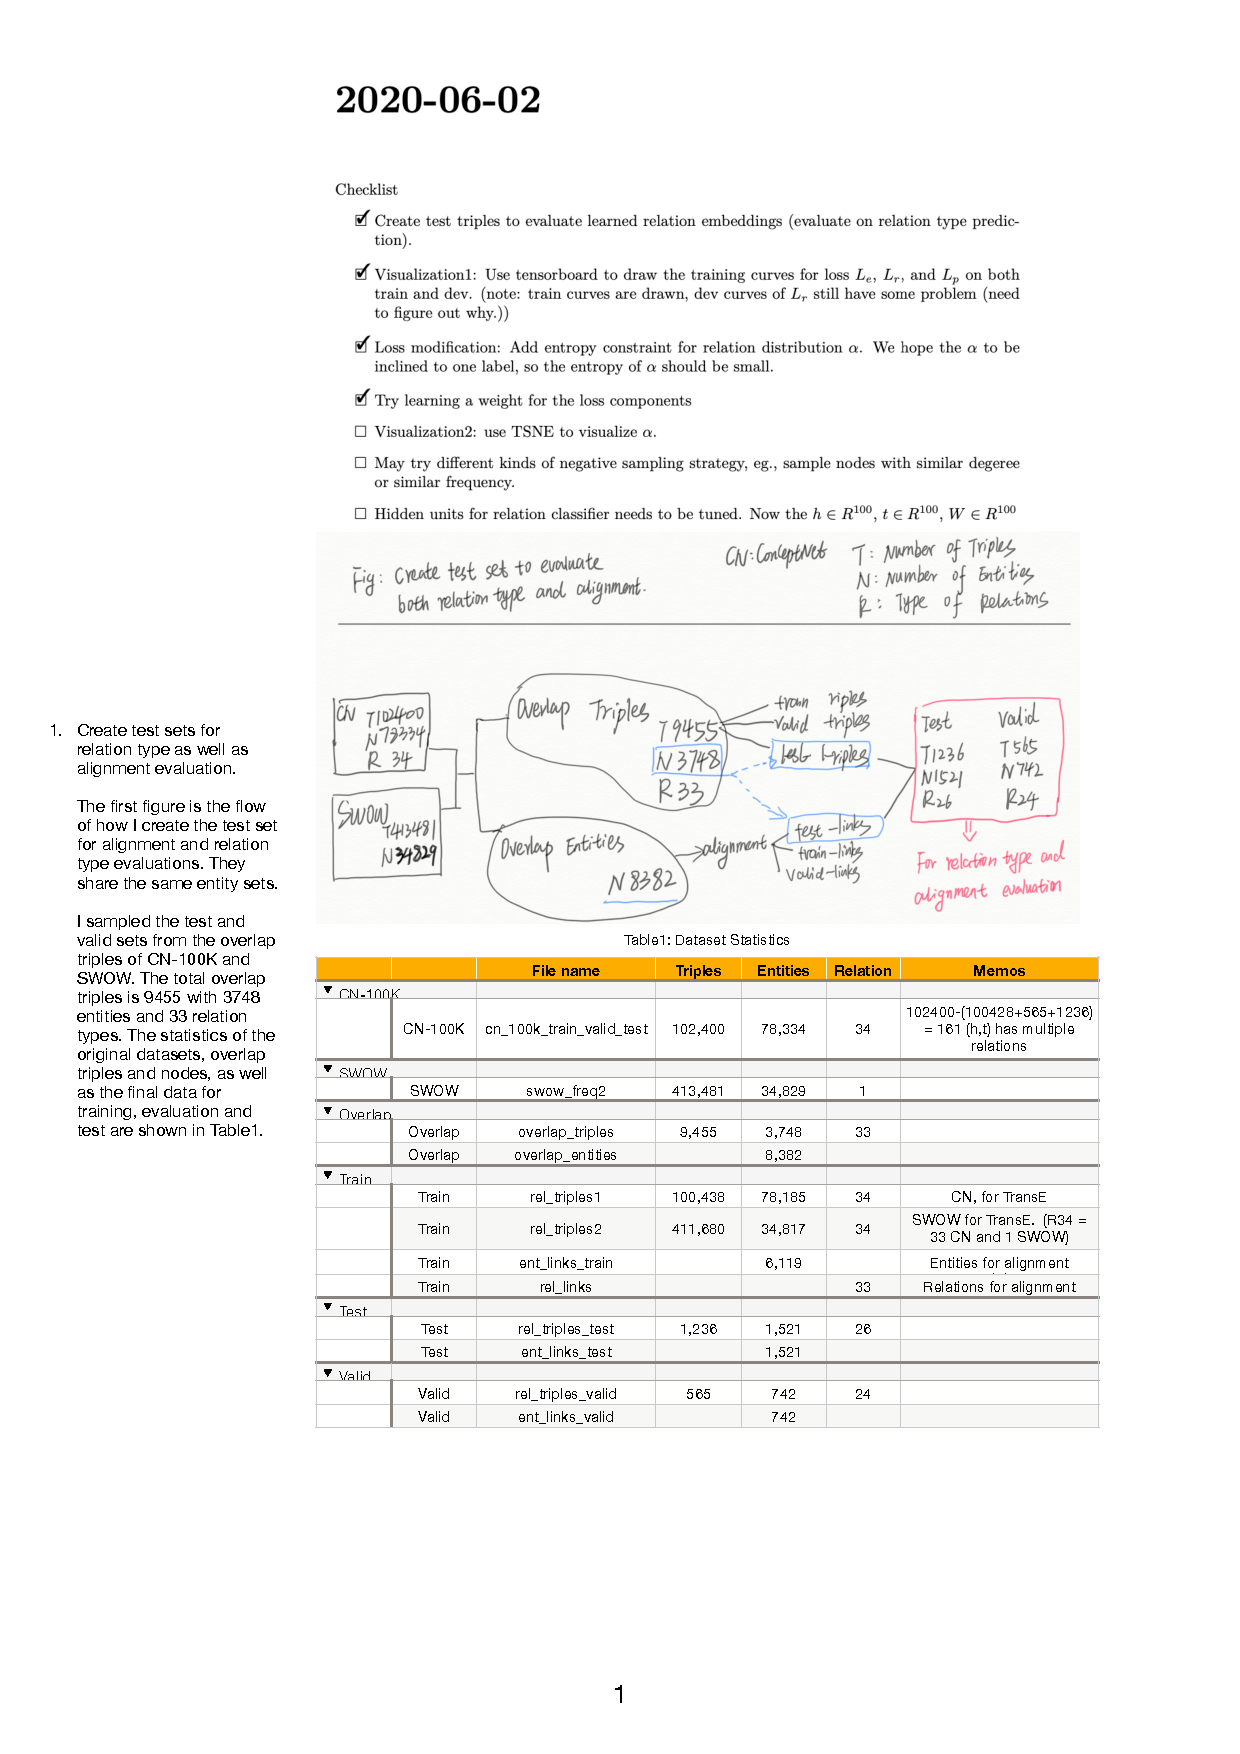
\includepdf[]{images/2020-06-02.pdf}
\clearpage
\section{Meeting Notes}
\textbf{To do list}
\begin{enumerate}
    \item For valid sets:
        \begin{enumerate}
            \item Figure out why hits and mrr on valid set is much lower than test set. 
            \item Visualize training curves on valid set. 
        \end{enumerate}
    \item Add evaluation on link prediction ($p(t|h,r)$) and triple classification (p(h,r,t) whether a triple exists).
    \item Add one more baseline: add the relation calssifier on TransE model and evaluate it. 
    \item Analysis on $\beta_1$ and $\beta_2$: 
    \begin{enumerate}
        \item Zoom in current $\beta_1$ (0-0.1) and $\beta_2$ (0.1-0.2) to see how they influce the MRR and the  REL\_ACC 
        \item Scale up the $\beta_1$ and $\beta_2$ to balance the scale range between $L_r$ and $L_p$ with $L_e$. (Because $L_e \approx 5*L_r$ and $L_e \approx 10*L_p$.) 
        \item Draw the correlation between $\beta_1$ and $\beta_2$ with the evaluation matrics. Observe how $\beta_1$ and $\beta_2$ influence the MRR or REL\_ACC.
    \end{enumerate}
    \item Print the confusion matrix for relation types to observe how model performs on each type.
    \item Apply dropout to model to tackle the overfitting problem of relaiton type accuracy.  
\end{enumerate} 
\chapter{2020-05-26}

\section{Learn SWOW relation types as a mixture of ConceptNet's relation}
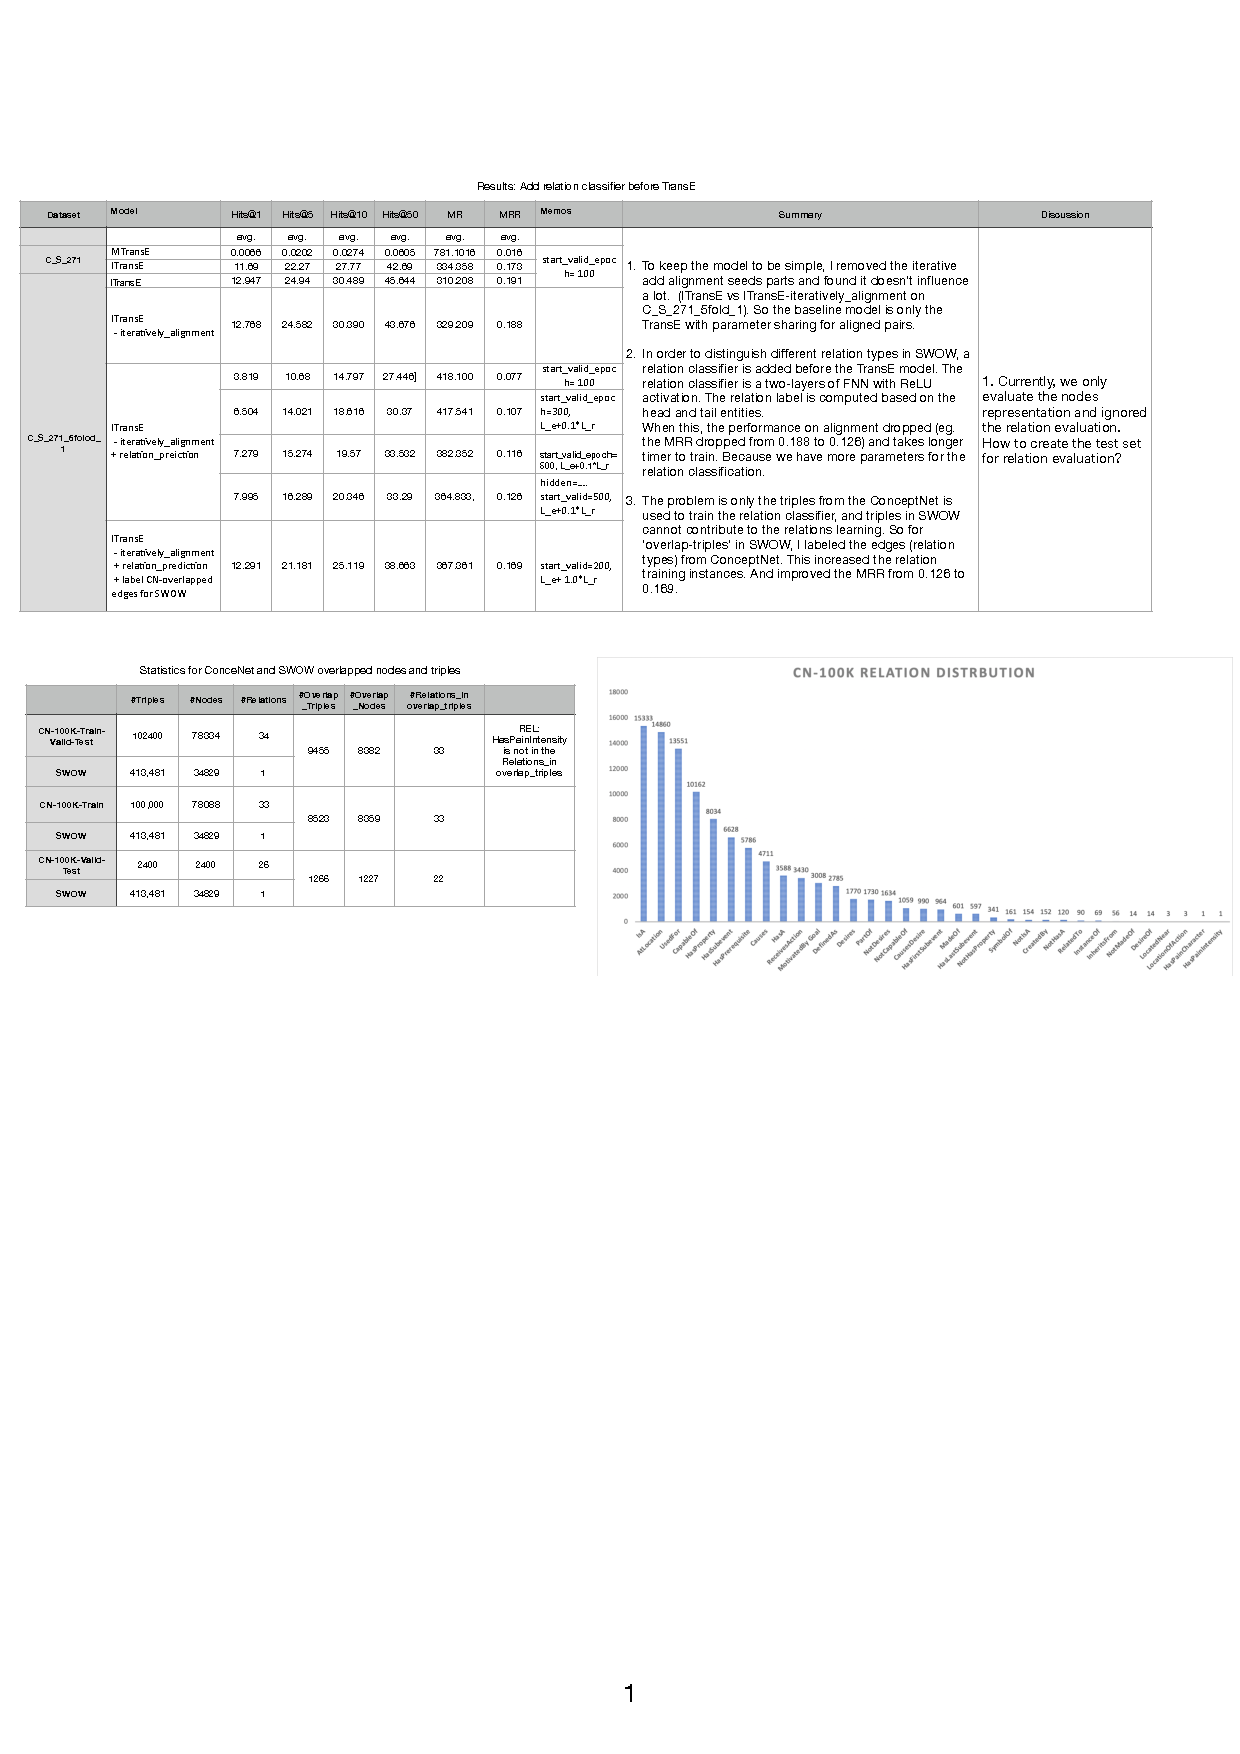
\includepdf[]{images/2020-05-26.pdf}

\section{Meeing Notes}
\textbf{To do list}
\begin{enumerate}
    \item Create test triples to evaluate learned relation embeddings (evaluate on relation type prediction).
    \item Loss modification: Add entropy constraint for relation distribution $\alpha$. We hope the $\alpha$ to be inclined to one label, so the entropy of $\alpha$ should be small. 
    \item Visualization: Use tensorboard to draw the training curves for loss $L_e$ and $L_r$, and use TSNE to visualize $\alpha$. (On both train and dev) 
    \item Maybe try different kinds of negative sampling strategy, eg., sample nodes with similar degeree or similar frequency. (But I am not really grasp why do we want this. How will this affect the model?)
   \item try learning a weight for the loss components
\end{enumerate}
Lea's comments: Regarding 4: we want this because by randomly sampling negative nodes we may make it too easy for the model to distinguish between true and fake triples. The fake ones will be completely implausible. We want to challenge the model by presenting it with plausible negative samples (somewhat like designing difficult multiple choice questions)

\begin{comment}
Relations id: {'LocationOfAction': 0, 'ReceivesAction': 1, 'HasPrerequisite': 2, 'MotivatedByGoal': 3, 'PartOf': 4, 'HasFirstSubevent': 5, 'HasProperty': 6, 'CreatedBy': 7, 'LocatedNear': 8, 'NotDesires': 9, 'HasSubevent': 10, 'DesireOf': 11, 'HasA': 12, 'InheritsFrom': 13, 'NotHasProperty': 14, 'HasPainIntensity': 15, 'CausesDesire': 16, 'RelatedTo': 17, 'NotMadeOf': 18, 'NotHasA': 19, 'InstanceOf': 20, 'Causes': 21, 'SymbolOf': 22, 'IsA': 23, 'HasPainCharacter': 24, 'UsedFor': 25, 'DefinedAs': 26, 'MadeOf': 27, 'AtLocation': 28, 'NotIsA': 29, 'NotCapableOf': 30, 'HasLastSubevent': 31, 'CapableOf': 32, 'Desires': 33} 

Relation counts from CN-100K (102400 triples total):

Relation count: [('HasPainCharacter', 1), ('HasPainIntensity', 1), ('LocatedNear', 3), ('LocationOfAction', 3), ('NotMadeOf', 14), ('DesireOf', 14), ('InheritsFrom', 56), ('
InstanceOf', 69), ('RelatedTo', 90), ('NotHasA', 120), ('CreatedBy', 152), ('NotIsA', 154), ('SymbolOf', 161), ('NotHasProperty', 341), ('HasLastSubevent', 597), ('MadeOf',
601), ('HasFirstSubevent', 964), ('CausesDesire', 990), ('NotCapableOf', 1059), ('NotDesires', 1634), ('PartOf', 1730), ('Desires', 1770), ('DefinedAs', 2785), ('MotivatedBy
Goal', 3008), ('ReceivesAction', 3430), ('HasA', 3588), ('Causes', 4711), ('HasPrerequisite', 5786), ('HasSubevent', 6628), ('HasProperty', 8034), ('CapableOf', 10162), ('Us
edFor', 13551), ('AtLocation', 14860), ('IsA', 15333)]



Loaded 377701 triples from ./data/alignment/C_S/rel_triples_1 with 30391 vocab
Total 37 relations.  Relation count: [('InstanceOf', 1), ('influencedBy', 1), ('SymbolOf', 3), ('EtymologicallyDerivedFrom', 6), ('NotCapableOf', 24), ('LocatedNear', 28), ('DefinedAs', 38), ('NotHasP
roperty', 112), ('CreatedBy', 135), ('HasFirstSubevent', 138), ('HasLastSubevent', 150), ('MadeOf', 281), ('CausesDesire', 311), ('Entails', 316), ('ReceivesAction', 418), ('Motiv
atedByGoal', 455), ('NotDesires', 512), ('Desires', 563), ('HasA', 822), ('HasPrerequisite', 886), ('DistinctFrom', 895), ('HasSubevent', 938), ('CapableOf', 971), ('Causes', 1078
), ('HasProperty', 1932), ('PartOf', 3146), ('UsedFor', 3998), ('Antonym', 4227), ('MannerOf', 8128), ('SimilarTo', 8225), ('AtLocation', 9659), ('FormOf', 11862), ('DerivedFrom',
 12778), ('IsA', 26499), ('HasContext', 30157), ('Synonym', 35660), ('RelatedTo', 212348)]


 Write 33 shared relations to ./data/alignment/C_S/rel_links                                                                                                               [51/1931]
Rel_links: {'Causes': 200, 'UsedFor': 1158, 'CausesDesire': 44, 'IsA': 2415, 'HasProperty': 1043, 'HasA': 326, 'MadeOf': 228, 'AtLocation': 2359, 'ReceivesAction': 147, 'PartOf': 
593, 'HasSubevent': 132, 'LocatedNear': 3, 'CapableOf': 280, 'NotCapableOf': 12, 'NotMadeOf': 4, 'HasLastSubevent': 12, 'InheritsFrom': 24, 'Desires': 65, 'HasPrerequisite': 136, 
'SymbolOf': 62, 'RelatedTo': 42, 'NotHasProperty': 32, 'MotivatedByGoal': 18, 'DefinedAs': 26, 'NotIsA': 19, 'CreatedBy': 35, 'NotDesires': 18, 'HasFirstSubevent': 3, 'LocationOfA
ction': 3, 'InstanceOf': 9, 'NotHasA': 4, 'DesireOf': 2, 'HasPainCharacter': 1}
\end{comment}

\chapter{2020-05-19}

\begin{comment}

\noindent \textbf{To do List}: 
\begin{todolist}

    \item List the difference of settings between our scenario and the ITransE \citep{Zhu2017IterativeEA}. 
    \item Try to see whether ITransE can apply to the alignments of ConceptNet and SWOW 
    \\(See does other people use their method in other bigger and sparser graph.)
\end{todolist}


\begin{todolist}
\item list our difference 
\item find out the baseline: fairly simple alignment methods, like for instance ITransE in its most vanilla version
    \begin{todolist}
    \item model architecture, losses
    \item input files, codes 
    \end{todolist}
\end{todolist}


TransE model, 
does any work on ConceptNet has used it before?

jointly train with alignment loss, iterative entity alignment


\begin{itemize}
    \item Project entities in two graph into one embeddings space, the training triples are 
\end{itemize}

\end{comment}

\begin{todolist}
\item[\done] set up openea environment
\item[\done] run IPTransE on datasets provided by \cite{Sun2020ABS}
\item[\done] read IPTransE code $\rightarrow$ convert to ITransE,

    \begin{todolist}
    \item[\done] delete \_generate\_path\_loss\
    %\item[\done] two graph one node embedding matrix and one rel matrix $\rightarrow$ two graphs two node embedding matrices, and two rel embedding matrices.
    \end{todolist}
\item[\done] read code: input file format
    \begin{todolist}
    \item[\done] read\_relation\_triples(): h r t
    \item[\done] aligned seed: test,train, valid=7:2:1
    \end{todolist}
\item[\done] prepare ConceptNet and SWOW aligned dataset 
\item[\done] run ITransE on ConceptNet and SWOW
\item read BootEA paper 
\item compare BootEA and ITransE
\item run BootEA or ITransE to see whether the results can match with the paper 
\end{todolist}


\section{Difference between Commonsense-cross-graphs and Others}

The first obvious difference is other graph are densier with less entity number and more relation types. Also, both graphs connected with a set of relation types. SWOW doesn't contain specific relation edges.

The second may be are nodes are non-canonicalized or free-form text, increasing the scale of graph. Also, may be this is why previous work used LSTM \citep{li-etal-2016-commonsense,Saito2018CommonsenseKB} instead of TransE to learn entity embeddings in commonsense knowledge graph.

(notes: I will be keep thinking about what is the biggest challenge of commonsense knowledge graph completion is, except for the sparsity?)
\begin{table}[htb]
    \centering
    \begin{tabular}{c|ccc}
    \hline
           dataset & \#Tiples &\#Ent  &\#Deg.  \\\hline
          DBP15K-EN & 101,058  & 14,984 &  13.49  \\
          DBP15K-FR & 93,016 & 14,991 & 12.41  \\
          WK3L-EN & 95,096 & 8,351 & 22.77  \\
          WK3L-FR & 68,787 & 7,180 & 19.16  \\
          \hline
          CN-100K & 100,000 & 78,088 & 1.25 \\
          SWOW & 413,481 & 34,831 &  11.77\\\hline
    \end{tabular}
    \caption{Statistics for various KGs. Sources come from \cite{Sun2020ABS} and \cite{Malaviya2019ExploitingSA}.}
    \label{tab:comparison-of-different-alignemnt-dataset}
\end{table}

\section{Experiments}
\subsection{Baseline models}
MTransE and ITransE are used as our baselines. 
\begin{table}[!ht]
    \begin{adjustbox}{max width=\textwidth}
    \centering
    \begin{tabular}{c|c|c|c}
          Model &  Embedding-loss $S_e$ & Align-loss $S_a$  & Iterative-loss $S_i$\\\hline
          MTransE &  $\sum\limits_{(h, r, t) \in T} E(h,r,t)$ & $\left\|\mathbf{M}^{e} \mathbf{e_1}-\mathbf{e_2}^{\prime}\right\|$  & 0 \\
          ITransE & $\sum\limits_{\left(h^{\prime}, r^{\prime}, t^{\prime}\right) \in T^{-}}\left[\gamma+E(h, r, t)-E\left(h^{\prime}, r^{\prime}, t^{\prime}\right)\right]_{+}$  & 0 & $\sum\limits_{\left(e_{1}, e_{2}\right) \in \mathbb{M}} R\left(e_{1}, e_{2}\right)\left(\mathcal{H}_{\left(e_{1}, e_{2}\right)}+\mathcal{H}_{\left(e_{2}, e_{1}\right)}\right)$ \\\hline
    \end{tabular}
    \end{adjustbox}
    \caption{Model losses, where $R\left(e_{1}, e_{2}\right)$ is a reliability score indicating how confident $e_1$ can be aligned to $e_2$.}
    \label{tab:model-losses}
\end{table}

\begin{align}
    & E(h, r, t)=\|\mathbf{h}+\mathbf{r}-\mathbf{t}\| \\
    & \mathcal{H}_{\left(e_{1}, e_{2}\right)}=\sum_{\left(e_{1}, r, t\right)} E\left(e_{2}, r, t\right)+\sum_{\left(h, r, e_{1}\right)} E\left(h, r, e_{2}\right)
\end{align}

Source code comes from OpenEA \cite{Sun2020ABS}. To ensure the provided code can achieve the performance reported in the original paper, I re-run the model on the cross-lingual entity alignment dataset EN-FR-15K-V1. The results (Table ~\ref{tab:results-on-en-fr-15k-v1} are pretty close to the reported results (Table 5 in \citep{Sun2020ABS}. So I applied them to align the ConceptNet and SWOW.

\subsubsection{Results on EN-FR-15K}
\begin{table}[!ht]
  \begin{adjustbox}{max width=\textwidth}
    \centering
    \begin{tabular}{@{}llllllllllllll@{}}
                               &                     & Hits@1 &        & Hits@5 &        & Hits@10 &        & Hits@50 &        & MR         &          & MRR    &        \\\hline
                               &                     & avg.   & std.   & avg.   & std.   & avg.    & std.   & avg.    & std.   & avg.       & std.     & avg.   & std.   \\\hline
\multirow{4}{*}{EN-FR-15K\_V1} & MTransE (reported)  & 0.2468 & 0.0056 & 0.4672 & 0.0086 & 0.5640  & 0.0093 & 0.7335  & 0.0160 & 251.9440   & 27.4550  & 0.3510 & 0.0070 \\
                               & IPtransE (reported) & 0.1690 & 0.0134 & 0.3204 & 0.0248 & 0.3903  & 0.0319 & 0.5289  & 0.0380 & 1,070.3200 & 136.4690 & 0.2430 & 0.0190 \\
                               & MTransE (re-run)    & 0.2498 & 0.0087 & 0.4680 & 0.0130 & 0.5637  & 0.0146 & 0.7328  & 0.0119 & 252.6916   & 13.5268  & 0.3528 & 0.0103 \\
                               & IPtransE (re-run)   & 0.1595 & 0.0111 & 0.3097 & 0.0215 & 0.3769  & 0.0252 & 0.5136  & 0.0275 & 1121.3191  & 111.3839 & 0.2323 & 0.0161\\\hline
\end{tabular}
\end{adjustbox}
\caption{Results on EN-FR-15K-V1.}
\label{tab:results-on-en-fr-15k-v1}
\end{table}

\subsection{Conceptnet-SWOW Alignment}
\subsubsection{Data Creation}
For both ConceptNet and SWOW, all the train, valid and test datasets are combined together to get the aligned entity seeds. The alignment is based on the string match, which generates 8,382 pairs of aligned entities. The statistics of source ConceptNet and SWOW are shown in Table~\ref{tab:concpetnet-swow-source-statistics}.
\begin{table}[!h]
    \centering
    \begin{tabular}{c|cccc}
    \hline
         Dataset &  edges	  & nodes&	overlaped\_nodes &	overlaped\_edges (one\_hop) \\\hline
        CN-100K &	102,400   &78,334 &	8,382 (10.70\%)	& 123,04 (12.01\%) \\
        SWOW & 413,481 &	34,831 &  8,382 (24.07\%)	& 123,04 (2.976\%) \\\hline
    \end{tabular}
    \caption{ConceptNet and SWOW source statistics}
    \label{tab:concpetnet-swow-source-statistics}
\end{table}

After that, the 8,382 pairs are split into test, train, and valid sets to train the model. Five-cross validation are used to train the model by following \cite{Sun2020ABS}. Two version of split are created, shown in Table~\ref{tab:c-s-721-271}.
\begin{table}[!ht]
    \centering
    \begin{tabular}{c|ccc}
    \hline
         DataSplits &  Test	 &  Train &	Valid 	\\\hline
         C\_S\_721 &5,868	 & 1,676   &838	  \\
         C\_S\_271 &1,676     &5,868 	 &  838 \\\hline
    \end{tabular}
    \caption{ConceptNet and SWOW source statistics.}
    \label{tab:c-s-721-271}
\end{table}

\subsubsection{Baseline Results}
\begin{table}[!h]
\begin{adjustbox}{max width=\textwidth}
\begin{tabular}{@{}llllllllllllll@{}}
                           &         & Hits@1 &        & Hits@5 &        & Hits@10 &        & Hits@50 &        & MR        &         & MRR    &        \\\hline
                           &         & avg.   & std.   & avg.   & std.   & avg.    & std.   & avg.    & std.   & avg.      & std.    & avg.   & std.   \\\hline
\multirow{2}{*}{C\_S\_721} & MTransE & 0.001  & 0.0003 & 0.0034 & 0.0003 & 0.0065  & 0.0003 & 0.0226  & 0.0012 & 2749.9197 & 16.1273 & 0.0038 & 0.0002 \\
                           & ITransE & 0.0084 & 0.0021 & 0.0264 & 0.0041 & 0.0397  & 0.0048 & 0.0905  & 0.0076 & 1994.6643 & 69.0998 & 0.0203 & 0.0029 \\ \hline
C\_S\_271                  & MTransE & 0.0066 & 0.0027 & 0.0202 & 0.0046 & 0.0274  & 0.0044 & 0.0605  & 0.0062 & 781.1016  & 11.1268 & 0.0159 & 0.0034 \\
                           & ITransE & 0.1169 & 0.0215 & 0.2227 & 0.0317 & 0.2777  & 0.0409 & 0.4269  & 0.0447 & 334.358   & 42.8182 & 0.1732 & 0.0264 \\\hline
\end{tabular}
\end{adjustbox}
\caption{Results on ConceptNet-SWOW aligned datasets.}
\label{tab:baseline-results-cs721-271}
\end{table}

It can be seen from the Table~\ref{tab:baseline-results-cs721-271} iterative update the aligned entity seeds indeed help the alignments. But the two models are different in many aspects. For example, the ITransE use negative sampling when learn node embeddings, and the current model use the parameter sharing mechanism to regularize the aligned entity pairs (that's why the align-loss in Table~\ref{tab:model-losses}.
These aspects may also influence the model. 

Besides, I will further observe how the model newly aligned entities looks like. 

\cite{Sun2020ABS} also show that BootEA \cite{sun-etal-2018-BootEa} is more good at align new entities, I will have a look at whether it is suitable for our situation.

\section{Meeting Notes}
\textbf{Discussion}
\begin{itemize}
    \item  Problem: TransE requires relation types to learn better embedding, but edges in SWOW is not labelled.
    \item  Solution: Cluster (h,t) pairs in SWOW so that TransE can differentiate different kind of relations.
\end{itemize}


\noindent \textbf{To do list}
\begin{enumerate}
    \item Figure out how to learn the cluster \\(I would be very appreciate if you can give me more hints about the methodology, still a little bit confusing how. Are we going to learn it jointly with the alignment or we design another model to learn it beforehand? Sorry that I don't have any practical cluster experience.)
    \item Verify the assumption that with clustered SWOW and ConceptNet, we can learn better alignment 
\end{enumerate}

\begin{comment}
% 28:00  Lea: use cocnept 
How do we use ConceptNet sensibly?  
use ConceptNet to distinguish the relations in SWOW, although we don't have it 
The relation types in ConceptNet can help us classify the SWOW relation types

30:40 Trevor 
Gating

34:40: cluster of relations type for SWOW 
every 
K random relations, each is a combinations of 

41:00
Talk about the alignment problem: SWOW has only 20\% of nodes in ConceptNet-100K but 80\% in Conceptnet5.7 

There could be 
\end{comment}


\begin{comment}
Miscellaneous: 
How to deal with the relation types in SWOW?
    \begin{itemize}
        \item use pre-trained language model (eg:Comet) to generate the relation types?
        \item  
    \end{itemize}
How to determine whether two triples are aligned or not? (where is the upper bound?)
How to select the training triples? (training graph)
\end{comment}
%Shared_entities:26703, take in ConceptNet: 0.8786 and SWOW: 0.7667 
%Aligned entities: test: 5341 train: 18692 valid: 2670

\begin{comment}
\subsection{Comments for ITransE}

Originally paper: Note that, since relations are universal and thus in this paper, we suppose all relations are already shared among various KGs.
ITransE requires all relations being shared among KGs. \cite{Zhu2017IterativeEA}

comments:\\
Because the approach
ITransE performs iterative alignment and it requires two KGs sharing the same relations, we
do not include it in the comparison.  \cite{wang-etal-2018-cross}


ITransE is used to align entities across
monolingual KGs with coherent vocabularies and triples, but
we find it does not adapt well to the inconsistent multilingual scenario.
ITransE works well on aligning coherent monolingual KGs [Zhu et al., 2017], but does
not adapt well to the inconsistent multilingual KGs. \cite{Chen2018CotrainingEO}

IPTransE fails to achieve good performance,
because it involves many errors as the self-training continues
but does not design a mechanism to eliminate these errors.
KDCoE propagates new alignment by co-training two orthogonal types of features, i.e., relation triples and textual
descriptions. However, this strategy does not bring improvement, due to some entities may lack textual descriptions. For
BootEA, it employs a heuristic editing method to remove
wrong alignment. After undergoing a period of fluctuations,
the precision stays stable while the recall continues growing
during self-training, which brings a clear performance boost.
Therefore, the design of semi-supervised learning strategies
has a strong influence on the final performance.
BootEA [21] adopts a bootstrapping approach
and iteratively labels the most likely alignments and utilizes them for further
training. In addition to the alignment loss, embeddings of aligned entities are
swapped regularly to calibrate embedding spaces against each other.

MTransE [5] learns a linear transformation between the embedding spaces of the individual graphs using L2-loss

IPTransE [29] embeds both KGs into the
same embedding space and uses a margin-based loss to enforce the embeddings
of aligned entities to become similar. 

\begin{table}[!h]
\begin{adjustbox}{max width=\textwidth}
    \begin{tabular}{l|llll|llll}
        & \multicolumn{4}{c|}{CN-100K}  & \multicolumn{4}{c}{SWOW}     \\\hline
       & MRR  & HITS@1 & HITS@3     & HITS@10
       & MRR  & HITS@1   & HITS@3   & HITS@10    \\\hline
MTransE   & 0.2980   & 0.2125  & 0.3304  & 0.4750   & -    & - & - & - \\
ITransE & 0.2942 \pm 0.0084 & 0.2078 \pm 0.0093 & 0.3254 \pm 0.0105 & 0.4736 \pm 0.0054 & 0.1816 \pm 0.0030&	0.1157 \pm 0.0029&	0.1924 \pm 0.0027&	0.3141  \pm0.0059  \\ 
        \hline                
    \end{tabular}
    \end{adjustbox}
    \caption{Results from baseline model GCN\_CONVTRANSE.}
    \label{Tab:GCN-CONVTRANSE-baseline}
\end{table}

Shared_vocab:8382, take in ConceptNet: 0.1070 and SWOW: 0.2407 
\end{comment}
\chapter{2020-05-12-Discuss ITransE}

\section{Model Architecture}
There are two assumptions in our idea: 
\begin{enumerate}
    \item The cross-graph neighbours representation augmentation is helpful.
    \item Aligned entities can supervise the training.
\end{enumerate}
In this week, I am focusing on the first assumption. The model architecture can be seen from Figure \ref{fig:model_architecture_2020_0512}. 
\begin{figure}[!ht]
    \centering
    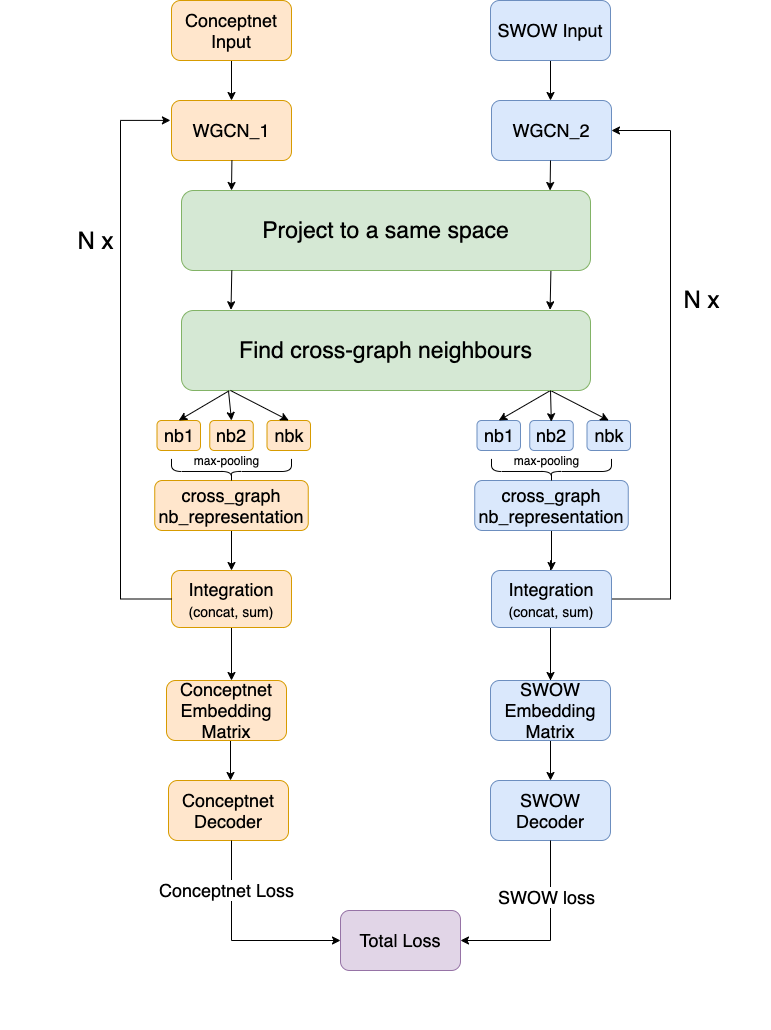
\includegraphics[scale=0.4]{images/0512/model-architecture-2020-05-12.png}
    \caption{Model Architecture}
    \label{fig:model_architecture_2020_0512}
\end{figure}

\section{Experimental Results}
The experimental results are shown in Figure\ref{fig:experimental_results}. 
\begin{figure}
    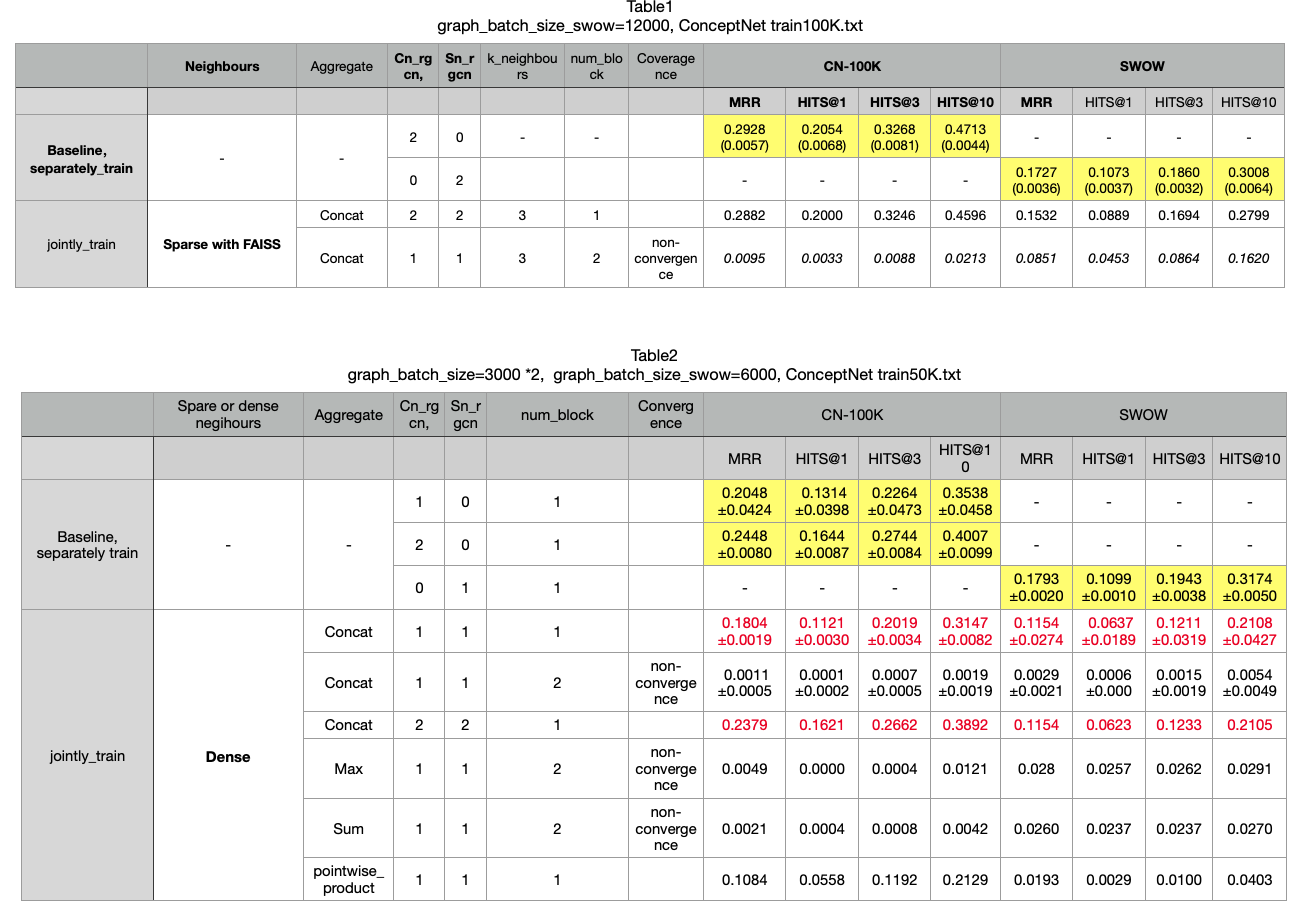
\includegraphics[scale=0.36]{images/0512/results-2020-05-12.png}
    \caption{Experimental Results}
    \label{fig:experimental_results}
\end{figure}

Table1 is the results of using FAISS to retrieve the topk nearest neighbours and get a vector representation for them with max-pooling. 
Table2 is replace the neighbour representation with the attention weight from $A=E_c E_s^T$. The ConceptNet training set in Table2 is decreased from 100K to 50K, because of the memory is not enough for the two big embedding matrix to multiply. Also, the graph\_batch\_size is decrease from 12,000 to 6,000. So the numbers will be different.

When block\_num is 1, I was trying to test whether the cross-graph neighbours representation can introduce extra knowledge and increase the performance. Compared with the baseline results, which is separately trained in each graph, the results of jointly training dropped. 

When block\_num is set to 2, I was trying to see whether stack the block multiple times can help the cross-graph neighbours be fused better. However, in both scenario, the model cannot converge. My guess is 1) it's too hard for the RGCN to aggregate both neighbours from its own graphs and another graph. 2) The cross-graph contains too much noise. 

So, for now, the experimental results are negative. 
\newpage
\section{Cross-graph Attention Related Work}

\cite{cao-etal-2019-multi} generate the cross-graph attention matrix to replace the adjacency matrix of GNN. The attention weight is for selecting neighbours in its own graph instead of the another graph. Their goal is to make the two sub-graphs from two different knowledge graph to share more common edges. 
\begin{align}
    \alpha_{i j}=\max _{r \in R, r^{\prime} \in R^{\prime}} \mathbf{1}\left(\left(e_{i}, r, e_{j}\right) \in T\right) \operatorname{sim}\left(r, r^{\prime}\right)
\end{align}
The attention matrix requires to compute the similarity between relation types of two graphs. However, it's not suitable for our research, because relation types in ConceptNet and SWOW are completely different. 

\cite{xu-etal-2019-cross-lingual} computes the attention matrix for each node in $G_{1}$ over all the nodes in $G_{2}$ and then combine them with the original nodes representation using a  multi-perspective cosine matching function $f_m$ before feeding them to a GCN. 
\begin{align}
    \alpha_{i, j}=\operatorname{cosine}\left(\boldsymbol{e}_{i}^{1}, \boldsymbol{e}_{j}^{2}\right) \quad j \in\left\{1, \ldots,\left|G_{2}\right|\right\} \\
    \boldsymbol{m}_{i}^{a t t}=f_{m}\left(\boldsymbol{e}_{i}^{1}, \overline{\boldsymbol{e}}_{i}^{1}\right)
\end{align}
Their matching function $f_m$ is very complicated, so I only used the dense attention idea in this week's work. 

\section{Meeting Notes}

\textbf{High level view}: 
\begin{enumerate}
    \item Can we learn the alignments?
    \item Can we use aligned seeds to help learn better nodes representation?
    \item Can better alignments help us complete the knowledge graph? 
\end{enumerate}


\noindent \textbf{To do List}: 
\begin{enumerate}
    \item  Modify current model architecture, 
        \begin{itemize}
            \item insert another gcn to integrate the integrated representation.
            \item integrate the self-graph representation and cross-graph nb representation using gate mechanism. 
        \end{itemize}
        
    \item List the difference of settings between our scenario and the ITransE \citep{Zhu2017IterativeEA}. 
    \item Try to see whether ITransE can apply to the alignments of ConceptNet and SWOW 
    \\(See does other people use their method in other bigger and sparser graph.)
\end{enumerate}





\begin{comment}
\section{ToDo}
\begin{todolist}
    \item model architecture modification\\
        remove the second layer of gcn and add the aggregation representation of cross-nb with original graph representation
       \begin{enumerate}
       \item Encode input graph with a WGCN
       \item Retrieve cross-graph neighbours 
       \item Construct cross-graph neighbours representation 
       \item Integrate self-graph representation with cross-graph representation, eg: f(W[a,b])
       \item Feed the integrated representation to WGCN (share parameters with the encoder WGCN or not share)  and repeat 1 to N times 
      \end{enumerate}       
    \item add alignment loss for supervision
        \begin{todolist}
            \item find a reasonable way to do negative sampling
        \end{todolist}
\end{todolist}

\begin{table}[]
    \centering
    \begin{tabular}{c|c}
         b&\\
         & 
    \end{tabular}
    \caption{Experiment re}
    \label{tab:my_label}
\end{table}
baseline:
 1. jointly train ConceptNet and SWOW by simply adding their loss together. 
 
 our model: 

why would I want to retrieve the cross-graph neighbours? 
\begin{itemize}
    \item In general, we want to  a bidirectional knowledge transfer between ConceptNet and SWOW. 	
\item One way could be 1. encode two graphs separately 2. Align entities in two graphs. 3. Update the representation for aligned words with representations from two graphs. We have proved that this idea can bring slight improvements for both graphs. However, we also found the limitation of this idea is that the aligned entities are limited \ref{tab:overlap-conceptnet-swow}, which means only a limited number of nodes representation will be updated. 

If we want to update more nodes, we need to increase their intersection parts.  

allow more nodes in one graph to influence the update of node representation. (What is the potential problems behind this?) 


\item  align the words in two graphs and 
\item  The aligned pair seeds in ConceptNet and SWOW are limited. If we only use the 
\end{itemize}

 each other's nearest neighbours and construct a cross-network node representation together with original graph represen
 How to speed up the process of idea verification ?
 \begin{itemize}
     \item  Hyper parameter
      \begin{itemize}
         \item reduce graph\_batch\_size 
         \item reduce training\_epochs 
         \item increase learning\_rate
    \end{itemize}
     \item data
         \begin{todolist}
         \item[\xmark] 16-bit precision , apex (ony support V100, TiTAN V)
         \item data Loader?  \href{https://towardsdatascience.com/9-tips-for-training-lightning-fast-neural-networks-in-pytorch-8e63a502f565}{here}
           \end{todolist}
     \item code 
       
 \end{itemize}

I am thinking the improvements of \cite{Malaviya2019ExploitingSA} comes a lot from the BERT model. Nodes in valid and test are fine-tuned on BERT model, even though they cannot be trained through GCN.
\section{Papers: deep graph matching}
do they compute similarity between all the nodes of two graphs or only select top-k nearest neighbours 
how do they integrate the attentive-representation and the original representation? 
%看是否有人 用sparsemax 选择neighbours
Do they have negative sampling? How do they do? 
Recently, graph neura
networks have become a focus of research leading to various proposed deep graph matching techniques (Wang et al., 2019b; Zhang & Lee, 2019; Xu et al., 2019d; Derr et al., 2019). 
Wang et al. (2019b) use node-wise features in
combination with dense node-to-node cross-graph affinities, distribute them in a local fashion, and
adopt sinkhorn normalization for the final task of linear assignment


\begin{align}
    \mathbf{m}_{j \rightarrow i}=f_{\text {message }}\left(\mathbf{h}_{i}^{(t)}, \mathbf{h}_{j}^{(t)}, \mathbf{e}_{i j}\right), \forall(i, j) \in E_{1} \cup E_{2} \\
    \boldsymbol{\mu}_{j \rightarrow i}=& f_{\text {match }}\left(\mathbf{h}_{i}^{(t)}, \mathbf{h}_{j}^{(t)}\right)   \forall i \in V_{1}, j \in V_{2}, \text { or } i \in V_{2}, j \in V_{1} \\
    \mathbf{h}_{i}^{(t+1)}=f_{\mathrm{node}}\left(\mathbf{h}_{i}^{(t)}, \sum_{j} \mathbf{m}_{j \rightarrow i}, \sum_{j^{\prime}} \boldsymbol{\mu}_{j^{\prime} \rightarrow i}\right)

\end{align}
\end{comment}
\chapter{2020-05-05}
\date{ }

%\begin{document}

%\maketitle
%\date{28 April, 2020}
	
	

\section{To do}

 \begin{todolist}
    \item  Experimental results
     \item  Papers about graph alignments 
    \item[\done]  Review the code for the top10 prediction 
\end{todolist}

\subsection{Code Review}
\begin{enumerate}
    \item Non-convergence $\leftarrow$swow doesn't suitable for 4 layer gcn.
         Solutions:
        \begin{todolist}
            \item[\done]    1. reduce SWOW rgcn and gcn layers
            \item    2. Information only flows from SWOW to ConcepeNet, not reverse
        \end{todolist}
        
    \item K-neighbours module has problem. Solutions:
        \begin{todolist}
            \item[\done] 1. only use top1 neighbour
            \item 2. set distance threshold
           \item 3. swap neighbours 
           \item[\done] 4. control the ratio between first rgcn and top gcn
        \end{todolist}

    \item Add alignment regularization 

    Analysis:
    The build\_nb\_graph is called in each batch. So the cross-network graph is different at each batch, which generating chaos for the node's representation. 
    Solutions:
    \begin{todolist}
    \item call build\_nb\_graph at each epoch. The advantage is that in each epoch, the model is training on a same cross-network. 
    \item Use swap neighbours method to fix the cross-network graph during whole training. (which is equa
    \end{todolist}

\end{enumerate}

\subsection{Paper Reading}
 
    \begin{todolist}
      \item[\done] survey
        \begin{itemize}
            \item  \href{https://arxiv.org/pdf/2002.00388.pdf}{A Survey on Knowledge Graphs:
Representation, Acquisition and Applications} 
            \item  \href{https://arxiv.org/pdf/2003.07743.pdf}{A Benchmarking Study of
Embedding-based Entity Alignment for Knowledge Graphs}
            \item \href{https://arxiv.org/pdf/1911.08342.pdf}{Knowledge Graph Entity Alignment with Graph
Convolutional Networks: Lessons Learned}
        \end{itemize}
      \item MultiKE: \href{https://arxiv.org/pdf/1906.02390.pdf}{Multi-view Knowledge Graph Embedding for Entity Alignment} %Swapping
      \item[\done] \href{https://arxiv.org/pdf/1911.08936.pdf }{AliNet:Knowledge Graph Alignment Network with Gated Multi-hop
Neighborhood Aggregation (AAAI 2019}    %neighbour embedding
      \item \href{https://www.ijcai.org/Proceedings/2019/0574.pdf}{A Vectorized Relational Graph Convolutional Network for Multi-Relational Network Alignment (IJCAI 2019)}  %regularization (new, and code available)
      
      \end{todolist}

\section{Summary}
\begin{enumerate}
    \item The non-convergence problem is because of two reasons: 1) the gcn layers for swow is too many, 2) the neighbors for the second gcn layer are not selected. \cite{Sun2019KnowledgeGA} also shows that with the increase of gcn layers, the MRR and HITS@N decrease a lot, seen Figure~\ref{fig:more_gcn_less_mrr}. 
    \begin{figure}[!ht]
    \centering
    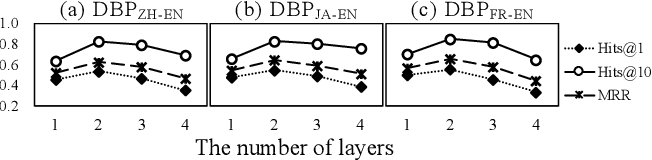
\includegraphics[scale=0.5]{images/0505/6-Figure4-1.png}
    \caption{With the increase of GCN layers, the MRR decreases a lot. From \cite{Sun2019KnowledgeGA}}
    \label{fig:more_gcn_less_mrr}
    \end{figure}

     \item About the neighbourhood selection 
      From the view of graph dendification. About graph densification, two kind of methods have been used.  \\
         1)  \textbf{Add training data explicitly}
         \begin{itemize}
             \item \textbf{Hard Selection}: Based on the assumption that an aligned pair of nodes should have similar neighbors in two kgs, some studies \citep{Ye2019AVR,Hu2019MultiKEAM,Zhu2019NeighborhoodAwareAR} 
        on graph alignment adopt the neighborhood swapping method to exchange the neighbors for aligned seed entities, and then add these generated triples back to the original graphs.  \\
        \item \textbf{Hard\&Soft}:
        \cite{Malaviya2019ExploitingSA} generate more training triplets by 1): selecting nodes with high similarities using the node's representations from a pre-trained BERT model, 2) adding reverse edges for all triples (directed graph directed graph $\rightarrow$  undirected graph). 
        Similarly, by arguing that distant (multi-hop) neighbors can also contribute to the entity alignment, \cite{Sun2019KnowledgeGA} allow distant neighbors together with direct neighbors (one-hop) to directly update the centered node representation. They use a gated mechanism to decide the importance of the distance neighbours and the direct neighbours. 
        \item{Rule-based} 
         MuGNN \citep{cao-etal-2019-multi} is the first paper I have read that jointly train KG completion and entity alignment. However, their completion module is based on rules, and they add margin loss to distinguish rule grounded triples and negative triples. 
         
        %现在的enetity alignment work ignored the heterogeneous structure problem. the core idea of this paper is generate similar structure for two nodes in two graphs by add missing edges and pruning irrelevant edges. It's the first I read that jointly train KG completion and entity alignment\\
        
    \end{itemize}
         2) \textbf{Cross-KG representation augmentation} \\
         For entities having fewer same neighbours in two graphs, GMNN \citep{xu-etal-2019-cross-lingual} claim that utilizing bilingual structure is better than monolingual structure information and thus formulate the problem of entity alignment as a graph matching problem by borrowing the idea from sequence matching. The bilingual representation is the concatenation of the original graph representation from a GCN and cross-KG attentive graph representation from its counterpart graph. \\
        This also can be seen as a kind of graph densification. 
        So basically, there are two options for the source of candidate neighbors: the original graph, and the another graph. So far, I haven't seen any papers combining both of them. 
           %\begin{table}[!h]
           %     \centering
           %     \begin{tabular}{c|c|c|c|c|c}
           %     \hline
           %         model &  source & soft\_or\_hard & selection\_method & inject\_at\_where & how\_to\_inject\\\hline
           %          & \\
           %     \hline
           %     \end{tabular} 
           %     \caption{Caption}
           %     \label{tab:my_label}
           % \end{table}
    \item  K-nearest neighbours 
         \begin{itemize}
             \item  The similarity distance from FAISS is decreasing with the training time increasing. It's hard to set up a fixed threshold directly to cut off the unimportant. This may cause  no neighbours are selected at the beginning of training. \\ 
             One possible way could be use the original neighbours at the beginning of training, and replace the neighbours when the model is warmed up.
             \item For now, I only choose the top1 nearest neighbour. (Still needs to figure out a better way.) This caused the \textit{hubness} problem, which means a hub of ponits frequently appear as the top-1 nearest neighbors of many other points. 
                \begin{table}[!ht]
                    \centering
                    \begin{tabular}{c|cccc}
                    \hline
                         Source&graph-type & \#Nodes & \#Edges & \#Shared\_Nodes \\  \hline
                         Original-Sub& ConceptNet &  7946 & 8000 & 1601 \\
                         & SWOW & 10467 & 8000 & 1601 \\
                         \hline
                         Cross-Sub & ConceptNet & 8246 & 7946&  \\
                            & SWOW & 12153 & 10467 & \\
                         \hline
                    \end{tabular}
                    \caption{\textit{Hubness} Problem caused by top1 nearest neighbour}
                    \label{tab:my_label}
                \end{table}
            \item  \textcolor{red}{TODO}: For now, the cross-network is generated in each batch. Intuitively, I don't think it's a good idea. So, generate a cross-network at each epoch seems to be more reasonable. 
            \item Nearest sampling has been used as negative sampling strategy \citep{sun-etal-2018-BootEa, cao-etal-2019-multi}. And negative samples are re-calculated every N epochs. 
         \end{itemize}
        
    
    \item About the alignment supervision \\
        Assumption: ``The assumption is that entities and their counterparts in different KGs should have similar structures and thus similar embeddings."
        \begin{itemize}
            \item Use $\gamma$ to control the ratio of alignment loss term. (The jointly loss has to be carefully balanced. $\leftarrow$ heterogeneous structure) 
            \item Distance inputs, project two embeddings to a shared space or not, $distance= f(Wa,Wb)$ , $distance=f(Wa,b)$ , $distance=f(Wa,b)$ or $distance=f(a,b)$, where $f$ could be L1 or L2 norm. 
            \item How to do negative sampling $(a,b)$ $a^{\prime}, b$ $a, b^{\prime}$ $a^{\prime}, b^{\prime}$
            \item \textcolor{red}{TODO}: Where to add the alignment loss? At the batch aligned entities or on the sub-graph aligned entities. (This may be a problem of my code, I add the sub-graph alignment loss on each batch training, that may influence triples not used in current training batch. I need to modify)
        \end{itemize}
\end{enumerate}


\section{Details about graph alignments }
Alignment supervision methods:
\begin{enumerate}
    \item Swap neighbors based on aligned entity seeds to generate more triples (More training data)  
    \item Minimize the distance between the aligned pairs and increase the distance between un-aligned pairs.  (Loss Function) \\
    AVR-GCN\citep{Ye2019AVR} combines both swapping and distance regularization and by splitting the aligned entities into two parts. 
\end{enumerate}

\noindent \textbf{Alignment}
maps entities into a unified representation space under
a joint embedding framework through aligned
translation as: 
    \begin{enumerate}
        \item aligned translation$\big |\big| e_1 + r^{(E1 \rightarrow E2)}  -  e_2 \big |\big|$   
        \item linear transformation as $M^{(E1\rightarrow E2)}e_1 - e_2$    
        \item parameter sharing as $e_1 \equiv e_2$.   
        \item parameter swapping: swaps seed entities in their triples to generate extra triples as supervision, $(e_1,r,e_2) \in \mathcal{G}_1$ $(e_1,r,e_2) \in \mathcal{G}_2$ 
    \end{enumerate}
    
    
\noindent\textbf{Distance Measure methods:}
\begin{align}
    & Manhattan: \big |\big|x -y \big |\big|_{L1} = \sum_{i=1}^{n} |x_i-y_i| \\
    & Euclidean:  \big |\big|x -y \big |\big|_{L2} = \sqrt{\sum\limits_{i=1}^{n} (x_i - y_i)^2} \\
    & Cosine(x,y) =  \frac{\sum_{i=1}^{n}x_i*y_i}{\sqrt{\sum_{i=1}^{n}{x_i}^2} \times \sqrt{\sum_{i=1}^{n}{y_i}^2}}  
\end{align}

%\textbf{Loss Function}


%\begin{comment}
\section{Details that may matter}

What's the key problem I am trying to solve?  \\
1. ConceptNet is sparse. So it's necessary to introduce some densification strategies to augment nodes with more neighbors?\\
2. The overlapping between ConceptNet and SWOW is small. If we are going to learn them jointly and allow more information flow from SWOW to ConceptNet, we need them to be tied deeper. 


How to pick neighbors for cross-network graph? Or how to generate cross-network?
 1. Generate dynamic cross-network graph.
 Where to train the cross-network graph? 
 Should we generate two cross-network graphs or only one?
 2. Swap neighbours of original two kgs for aligned entities.  
 
How to make use of aligned entities as supervision signals? 

%\end{comment}



\section{TopK Prediction Observation}
\begin{figure}[!ht]
    \centering
    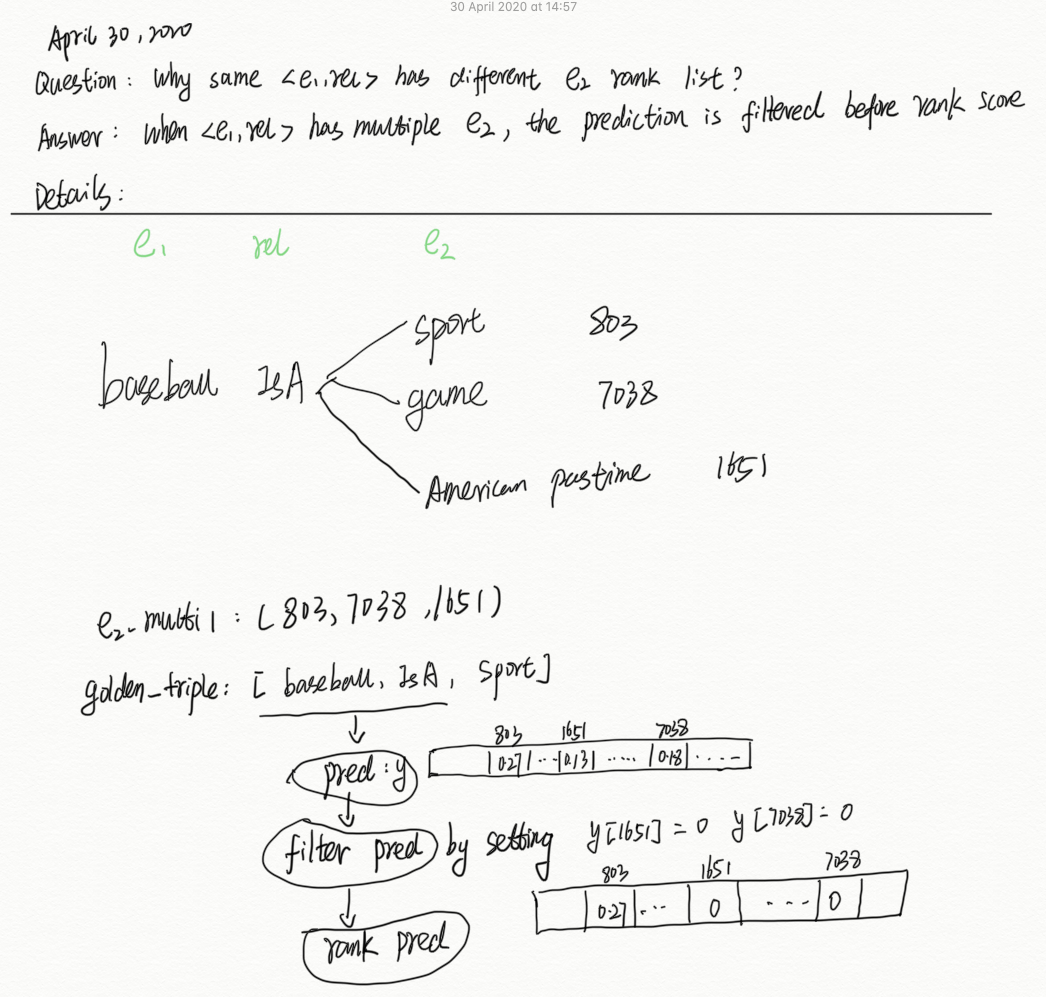
\includegraphics[width=\textwidth]{images/filter_prediction.png}
    \caption{Filter prediction before rank}
    \label{fig:my_filter_prediction}
\end{figure}

Lea: 
Yes, but why do you set "game" and "american passtime" to zero when evaluating [baseball, isA, sport]?

Chunhua: 
They say they follow the previous work. This is an updated version for compute MRR and HITS@N directly. For example, when we are evaluating the <baseball, IsA, sport> , if the score <baseball, IsA, game> is higher than the <baseball, IsA, sport>, then when computing the loss, the model would think this is a wrong prediction. But actually, it’s true. 

Originally from \href{https://papers.nips.cc/paper/5071-translating-embeddings-for-modeling-multi-relational-data.pdf}{Translating Embeddings for Modeling Multi-relational Data}


%\printbibliography
%\end{document}



\end{comment}

\chapter {2020-04-28}

%\begin{document}

%\maketitle
%\date{28 April, 2020}
To do list:
Problems: Speed and Debug
speed: backward process is very slow 

There are two places need to tensors copies between devices: GPU $\rightarrow$ CPU $\rightarrow $ GPU.  

The first one is when using FAISS to retrieve the neighbours, the ConceptNet and SWOW embedding matrix have to be copied from GPU to CPU. Because gpu tensors can not be input directly to the FAISS to build index, and search. After searching, these neighbour tensors have to be copied back to GPU.   

The second is when constructing and training new graphs. Currently, I am using the output embeddings from GCN to retrieve neighbours. So I have to construct the graph dynamically in each epoch. This process increases two graphs with more nodes to train. For example, if the nodes number of ConceptNet and SWOW is $N_C$ and $N_S$ respectively. Then the increased two graph nodes number would be $N_C^\prime \approx N_S + N_C $ and $N_S^\prime \approx N_S + N_C$

\begin{table}[!h]
    \centering
    \begin{adjustbox}{max width=\textwidth}
    \begin{tabular}{c|c|c|c|c}
    \hline
    & graph\_batch\_size & epoch\_time (minutes)  & forward\_batch\_time(s) & backward\_batch\_time(s) \\\hline
     Original & 12,000 $\times$ 2   & 0.83  & 0.0177 & 0.0896\\  \hline
     Now & 12,000 $\times$ 2 + 15,000 $\times$ 2  &  7.8333  & 0.0203 & 0.8505\\
     \hline
    \end{tabular}
    \end{adjustbox}
    \caption{Time consuming comparison}
    \label{tab:time-consume}
\end{table}


Which part slows down this process? Can you find a better method? 


\section{How to determine the parameters of IndexIVFFlat()}
%All IVF index work by splitting the vectors into nlist clusters, according to the quantizer. During search time, only nprobe clusters are searched.
There are two parameters to the search metho nlist, the number of cells, and nprobe, the number of cells (out of nlist) that are visited to perform a search. The search time roughly increases linearly with the number of probes plus some constant due to the quantization.  
\begin{enumerate}
    \item How to choose a suitable nlist?\\
If we have a matrix with n vectors, 4 * sqrt(n) is usually reasonable, or some other O(sqrt(n)). 
    \item How to choose a suitable nprobe?
    \item Hot to decide the number of neighbours? 
\end{enumerate}
	%\subsrction{how do I construct the new graph and train }


%\section{Current experimental time comparison}



\section{Code Details}

%Python code highlighting
\begin{lstlisting}[language=Python, caption=Python example]
import numpy as np
  def gpu_pytorch_neighbours(self, xb_t, xq_t):
         gpu_index_ivf = faiss.GpuIndexIVFFlat(self.res, self.d,\
                                               self.nlist, faiss.METRIC_L2)

         assert not gpu_index_ivf.is_trained
         xb_t = xb_t.detach().cpu().numpy()
         gpu_index_ivf.train(xb_t)        # faiss doesn't accept gpu tensors
         assert gpu_index_ivf.is_trained

         gpu_index_ivf.add(xb_t)

         D, I = search_index_pytorch(gpu_index_ivf, xq_t, self.k)

         return D, I
\end{lstlisting}


\clearpage
\section{Model Outputs}

I tried to compare the outputs of train one graph and jointly train two graphs. 
% if target in top10 prediction, how many examples is jointly train higher than separately train. 

% For the top10 predictions, jointly trained model prediction are more reasonable than separately train. 

% I can see two observations: 
% \begin{enumerate} 
  %   \item Jointly training increase the score of the top1 prediction. For 
% \end{enumerate}

\begin{table}[!h]
\begin{adjustbox}{max width=\textwidth}
\begin{tabular}{c|c|c|c|c}
    \hline
    Triple & ConceptNet Alone &rank & Jointly Train & rank \\\hline
    \{"e1": "do housework", "e2": "clean house", "relation": "Causes"\} & 	0.5661 & 	1 & 	0.6026	& 1 \\
     \{"e1": "pen", "e2": "write", "relation": "UsedFor"\} &	0.5554 &	1 &	0.4404	&1 \\
    \{"e1": "apple", "e2": "green", "relation": "HasProperty"\} & 0.1712 & 1 & 0.5432 & 1\\
     \{"e1": "bottle", "e2": "plastic", "relation": "MadeOf"\}	&	- & - &	0.0185	&9 \\
     \{"e1": "bottle", "e2": "glass", "relation": "MadeOf"\} &	0.1614 &	1&	0.0395&	2 \\\hline
\end{tabular}
\end{adjustbox}
\caption{Sampled top 10 predictions. - indicates the target is outside top10. }
\end{table}

Sampled a weird instance and a positive instance. 

\begin{figure}[!ht]
    \centering
    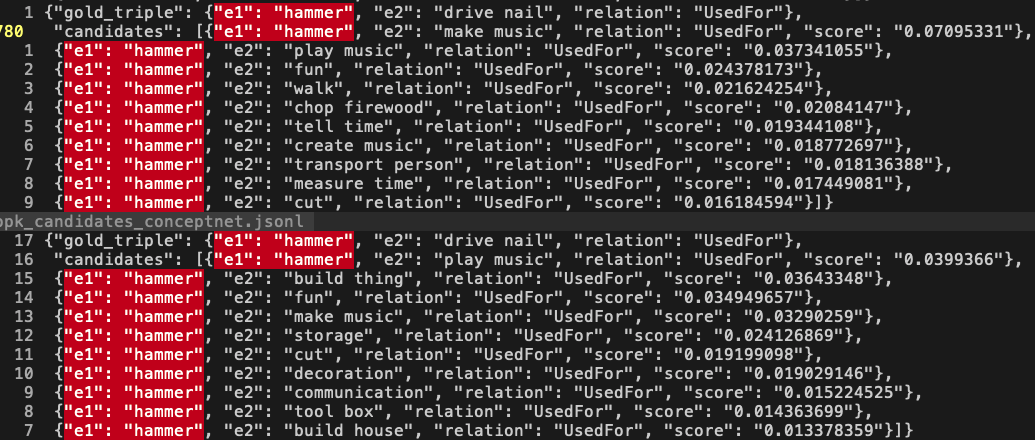
\includegraphics[scale=0.45]{images/hammer_top10_predictions.png}
    \caption{Hammer\_top10\_predictions. The top is from train ConceptNet alone and the bottom is from jointly training. Jointly train model is align before gcn embedding with pointwise pooling.}
    \label{fig:hammer-top10-prediction}
\end{figure}


The prediction files can be found at  \href{https://unimelbcloud-my.sharepoint.com/:f:/g/personal/chunhua_student_unimelb_edu_au/EuJ4GNdJNnFAmiDw7eE13oIBzBR7eJUrvyPRSEi8mrXIFw?e=bl9BcD}{here}
%\end{document}

\chapter{2020-04-21}
%\begin{document}

%    \maketitle
    
%    \begin{abstract}
        
%    \end{abstract}
    
%    \tableofcontents
 %   \thispagestyle{empty}
  %  \newpage
   % \setcounter{page}{1}
\section{Model Architecture}
\begin{figure}[!ht]
    \centering
    %\begin{adjustbox}{width=\textwidth}
   % \begin{adjustbox}{max width=\textwidth,height=8cm}
    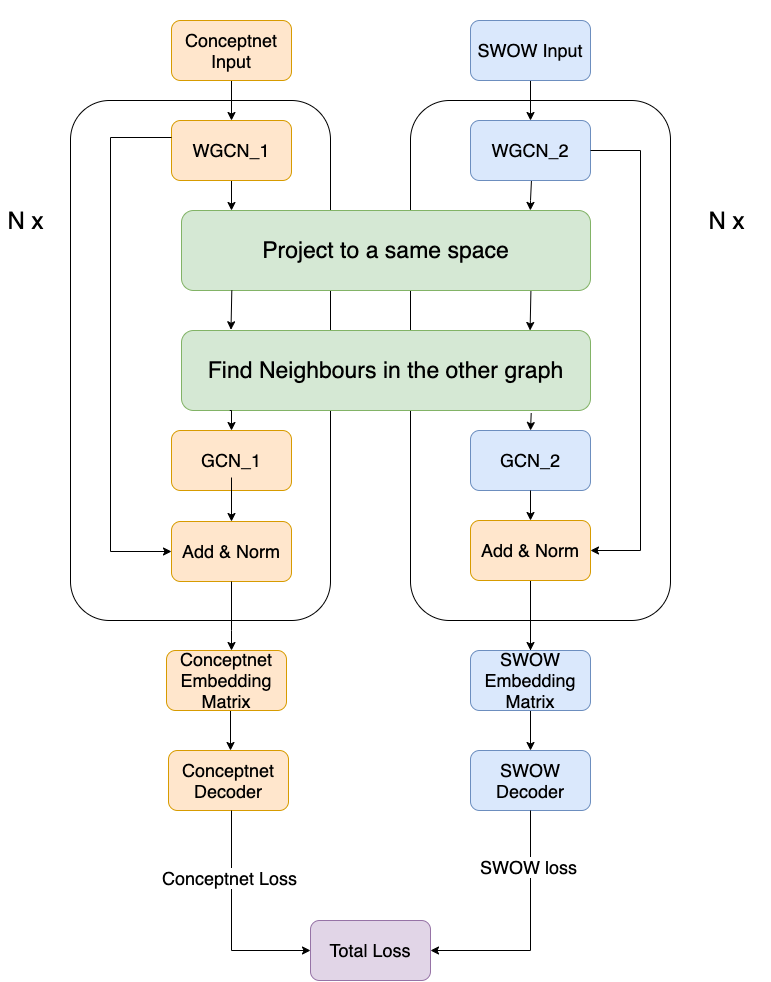
\includegraphics[scale=0.45]{images/conceptnet-swow.png}
   % \caption{Caption}
     \label{fig:concept-swow-model-architecture}
     %\end{adjustbox}
\end{figure}

In previous methods, the neighbours of a node in a graph are static or fixed, and will not updated during the whole training process. The core view of this idea is to update the neighbours of a node in the training process. In this way, we can compute the neighbours of a the node and thus gain a another embedding for this node. Then, for each node, we can combine the two embeddings with different weight to gain a new embedding.  For the sources of the neighbours, there can be two options, from the its own graph and another graph. If it is from its own graph, then it can be seen as the "self-attention" in Transformer. 
If it's from another graph, it can introduce more external knowledge. 
One thing needs to be noted is that we can only obtain the neighbour nodes, the edge label (relation type) information cannot be obtained. So the GCN for initial graph and updated graph will be a little bit different. Take the latter option for example, the process can be formulated with the following equations: \\

\noindent Notations: \\ 
C: the initial ConceptNet graph  (with initialized node embedding matrix, relation types, each node has initial neighbours)\\
S: the initial SWOW graph.  (similar as ConceptNet)
\\$C_n$: updated Concept graph with neighbours from SWOW (with nodes in original ConceptNet and also their embeddings. Each node has a set of neighbours, whose embeddings come from SWOW, no relation types) \\ 
$S_n$: updated SWOW graph with neighbours from ConceptNet. (similar to $C_n$)

\begin{align}
\mathbf{E_{c} } & = WGCN(C),  & \mathbf{E_{s}}  & = WGCN(S) \label{formula:gcn}\\
 \mathbf{E_{c}^m} & = f_m(\mathbf{E_c}), &  \mathbf{E_{s}^m} & =f_m(\mathbf{E_s}) \label{formula:prjection} \\
C_n  &= g(\mathbf{E_{c}^m}, \mathbf{E_{s}^m}),  & S_n  & = g(\mathbf{E_{s}^m}, \mathbf{E_{c}^m})   \label{formula:find_neighbours} \\
    \mathbf{E_c^{\prime}}& = GCN(C_n),   & \mathbf{E_s^{\prime}} & =GCN(S_n) \label{formula:gcn2} \\
    E_c^o  &= f_l(\mathbf{E_c } + \mathbf{E_c^{\prime}}), & E_s^o & = f_l(\mathbf{E_s } + \mathbf{E_s^{\prime}}),  \label{formula:layrnorm}
\end{align}
Equation~\ref{formula:prjection} uses function $f_m$ to project the two embedding matrices into a same space\\
Equation~\ref{formula:find_neighbours}  finds the neighbours in in each other's graph.\\
Equation~\ref{formula:gcn2} passes the new graph (neighbours are from another graph) to another gcn.\\
Equation~\ref{formula:layrnorm} adds the two embedding matrices from two gcn layer and performs a layernorm on them.


The above five equations will be wrapped as a whole and repeated many times. 

%\printbibliography


%\section{To do list}
%

%\end{document}



\bibliography{references}
\end{document}




